%%%%%%%%%%%%%%%%%%%%%%%%%%%%%%%%%%%%%%%%%%%%%%%%%%%%%%%%%%%%%%%%%%%%%%%%%%%
\section{Waves in a bounded ocean}
\label{SectionGraphic}
%%%%%%%%%%%%%%%%%%%%%%%%%%%%%%%%%%%%%%%%%%%%%%%%%%%%%%%%%%%%%%%%%%%%%%%%%%%

\subsection{Graphical investigation of Modified Surface Waves (MSW), Modified Acoustic Modes (MAM) and Modified Internal Modes (MIM)}
\label{SubSectionPotBranches}
The compressible and stratified ocean is now supposed to be bounded. Wave solutions must consequently satisfy both the inner \ref{EqFullDispera} and boundary \ref{EqFullDisperb} dispersion relations. In phase space, they must lie at the intersections of the inner and boundary dispersion surfaces, which are plotted simultaneously on Figure \oldref{FigDispSolutions}.
%
\paragraph{Branches of the boundary dispersion surface}
%
\begin{figure}[h]
	\centering
	\subfloat[][]{
	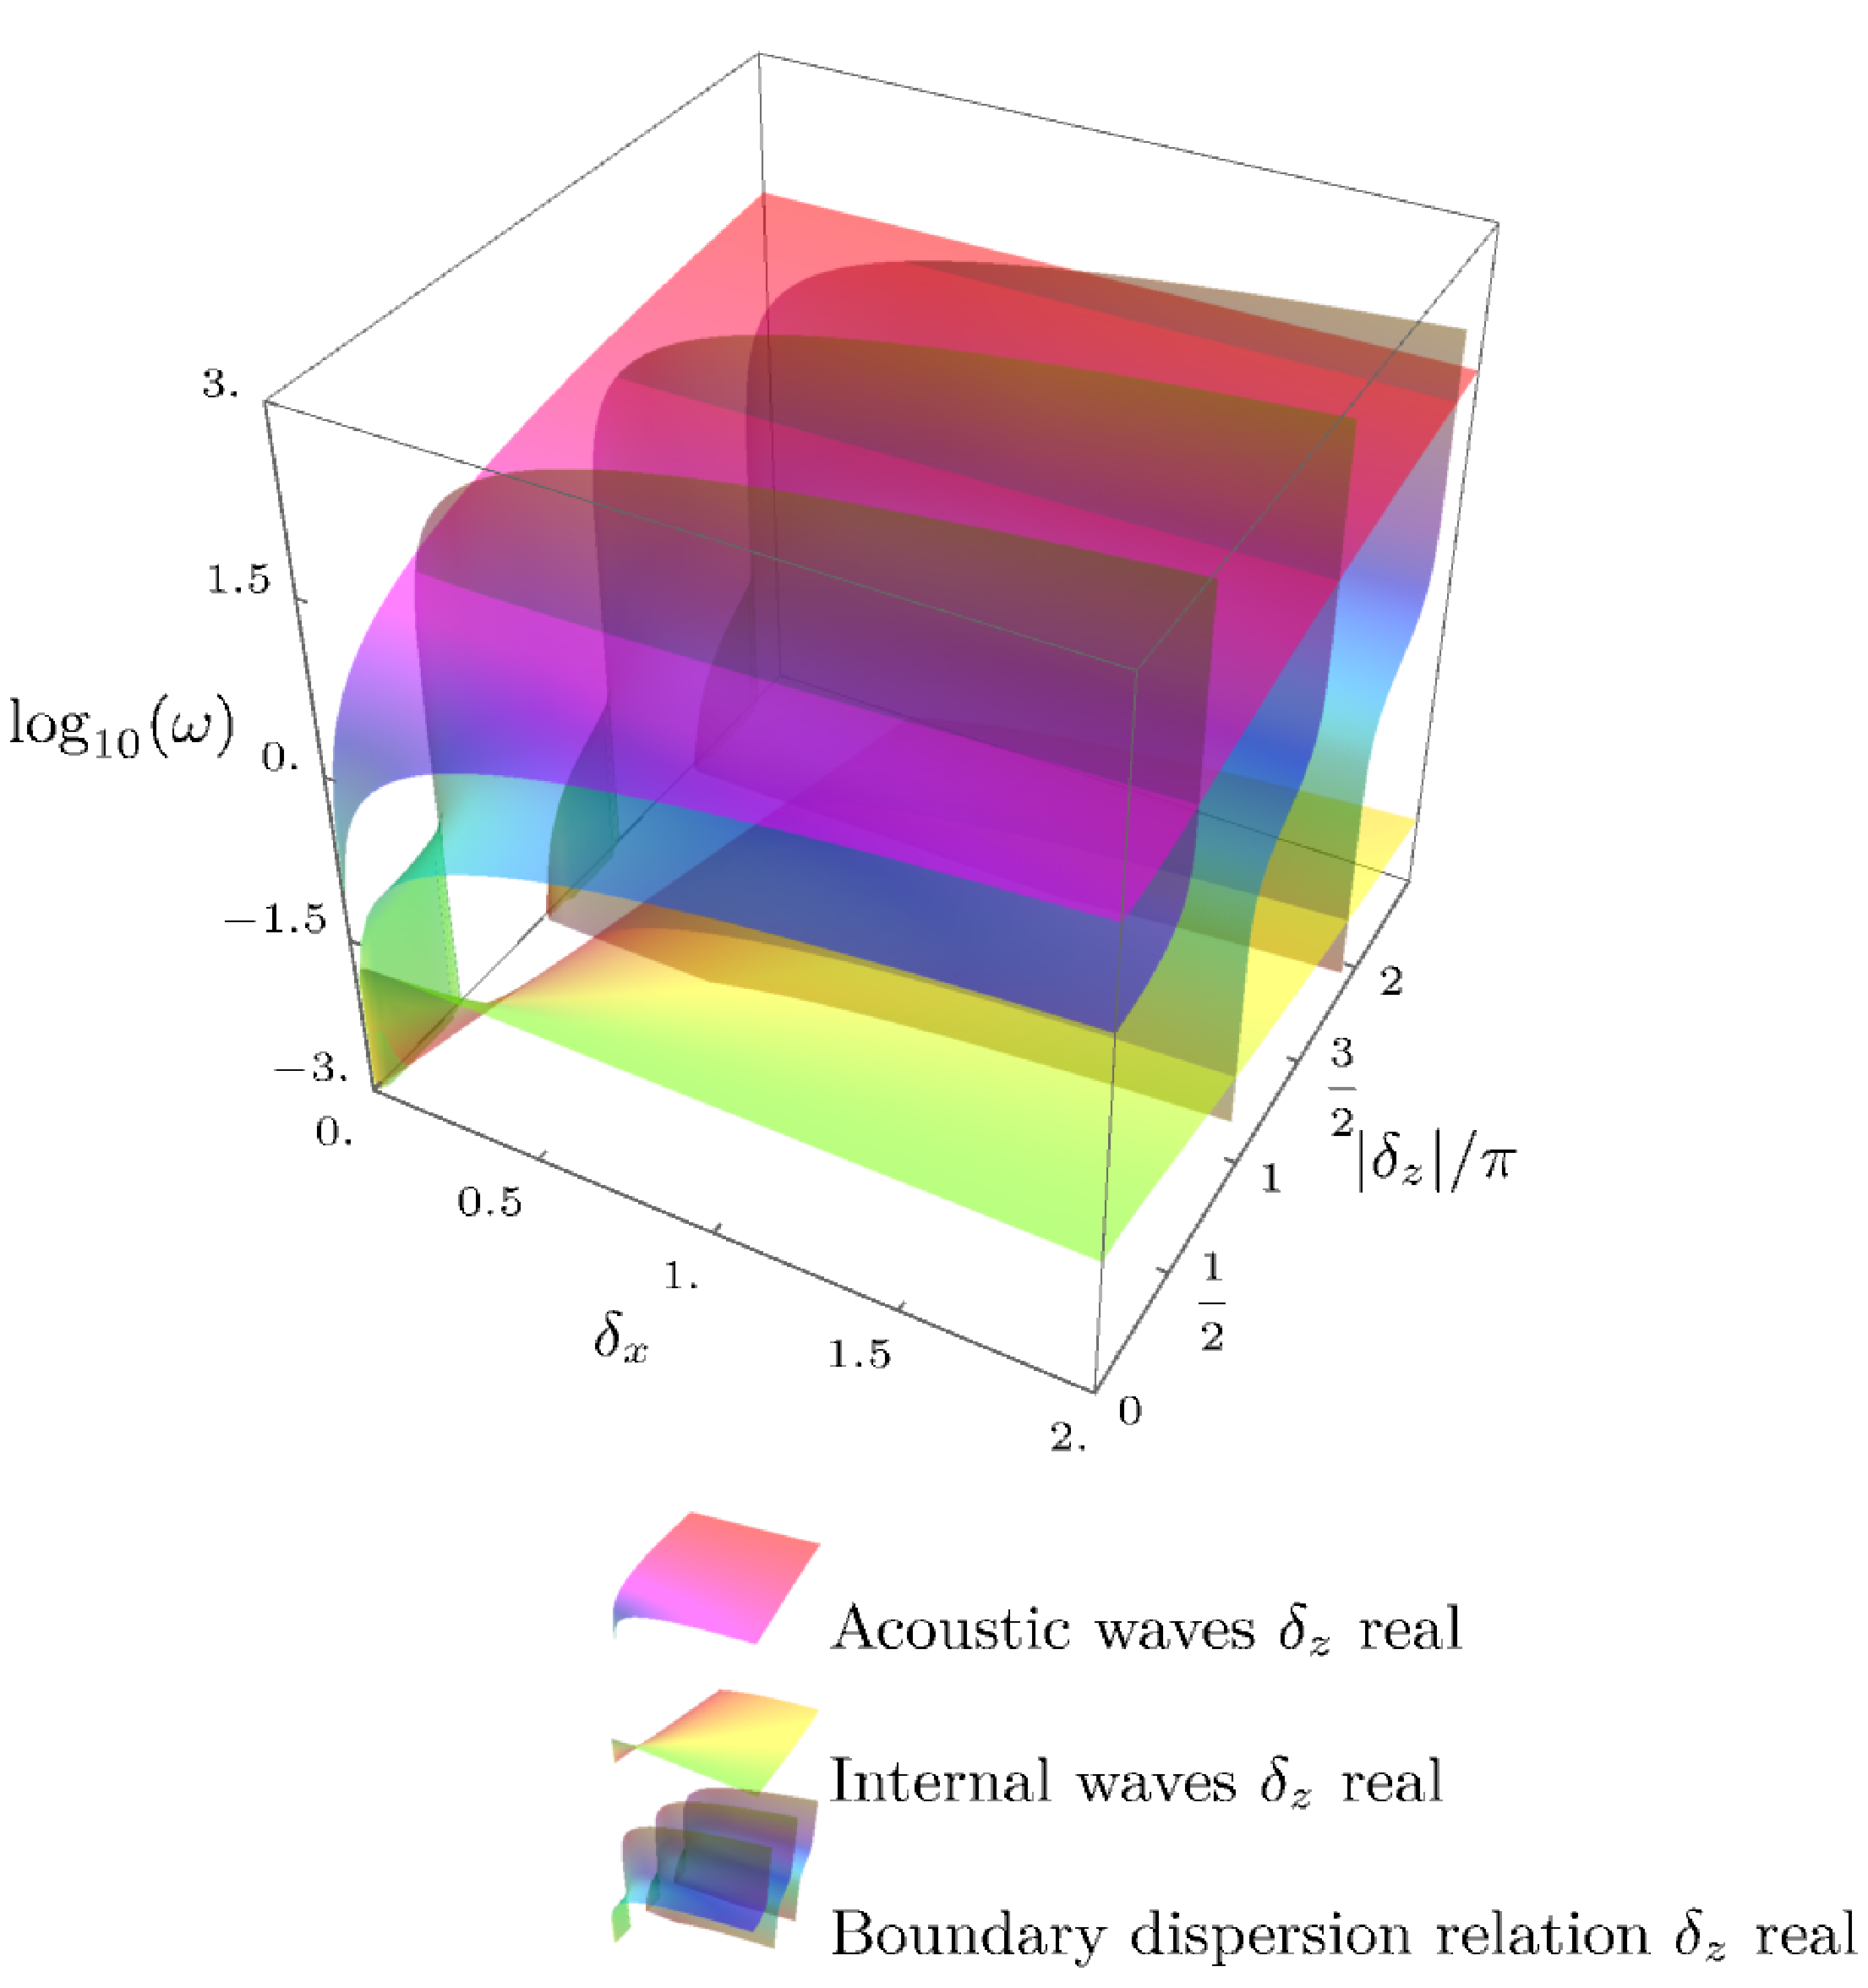
\includegraphics[width=0.45\linewidth]{FIGURES/boundedreal.png}
}
	\centering		
	\subfloat[][]{
		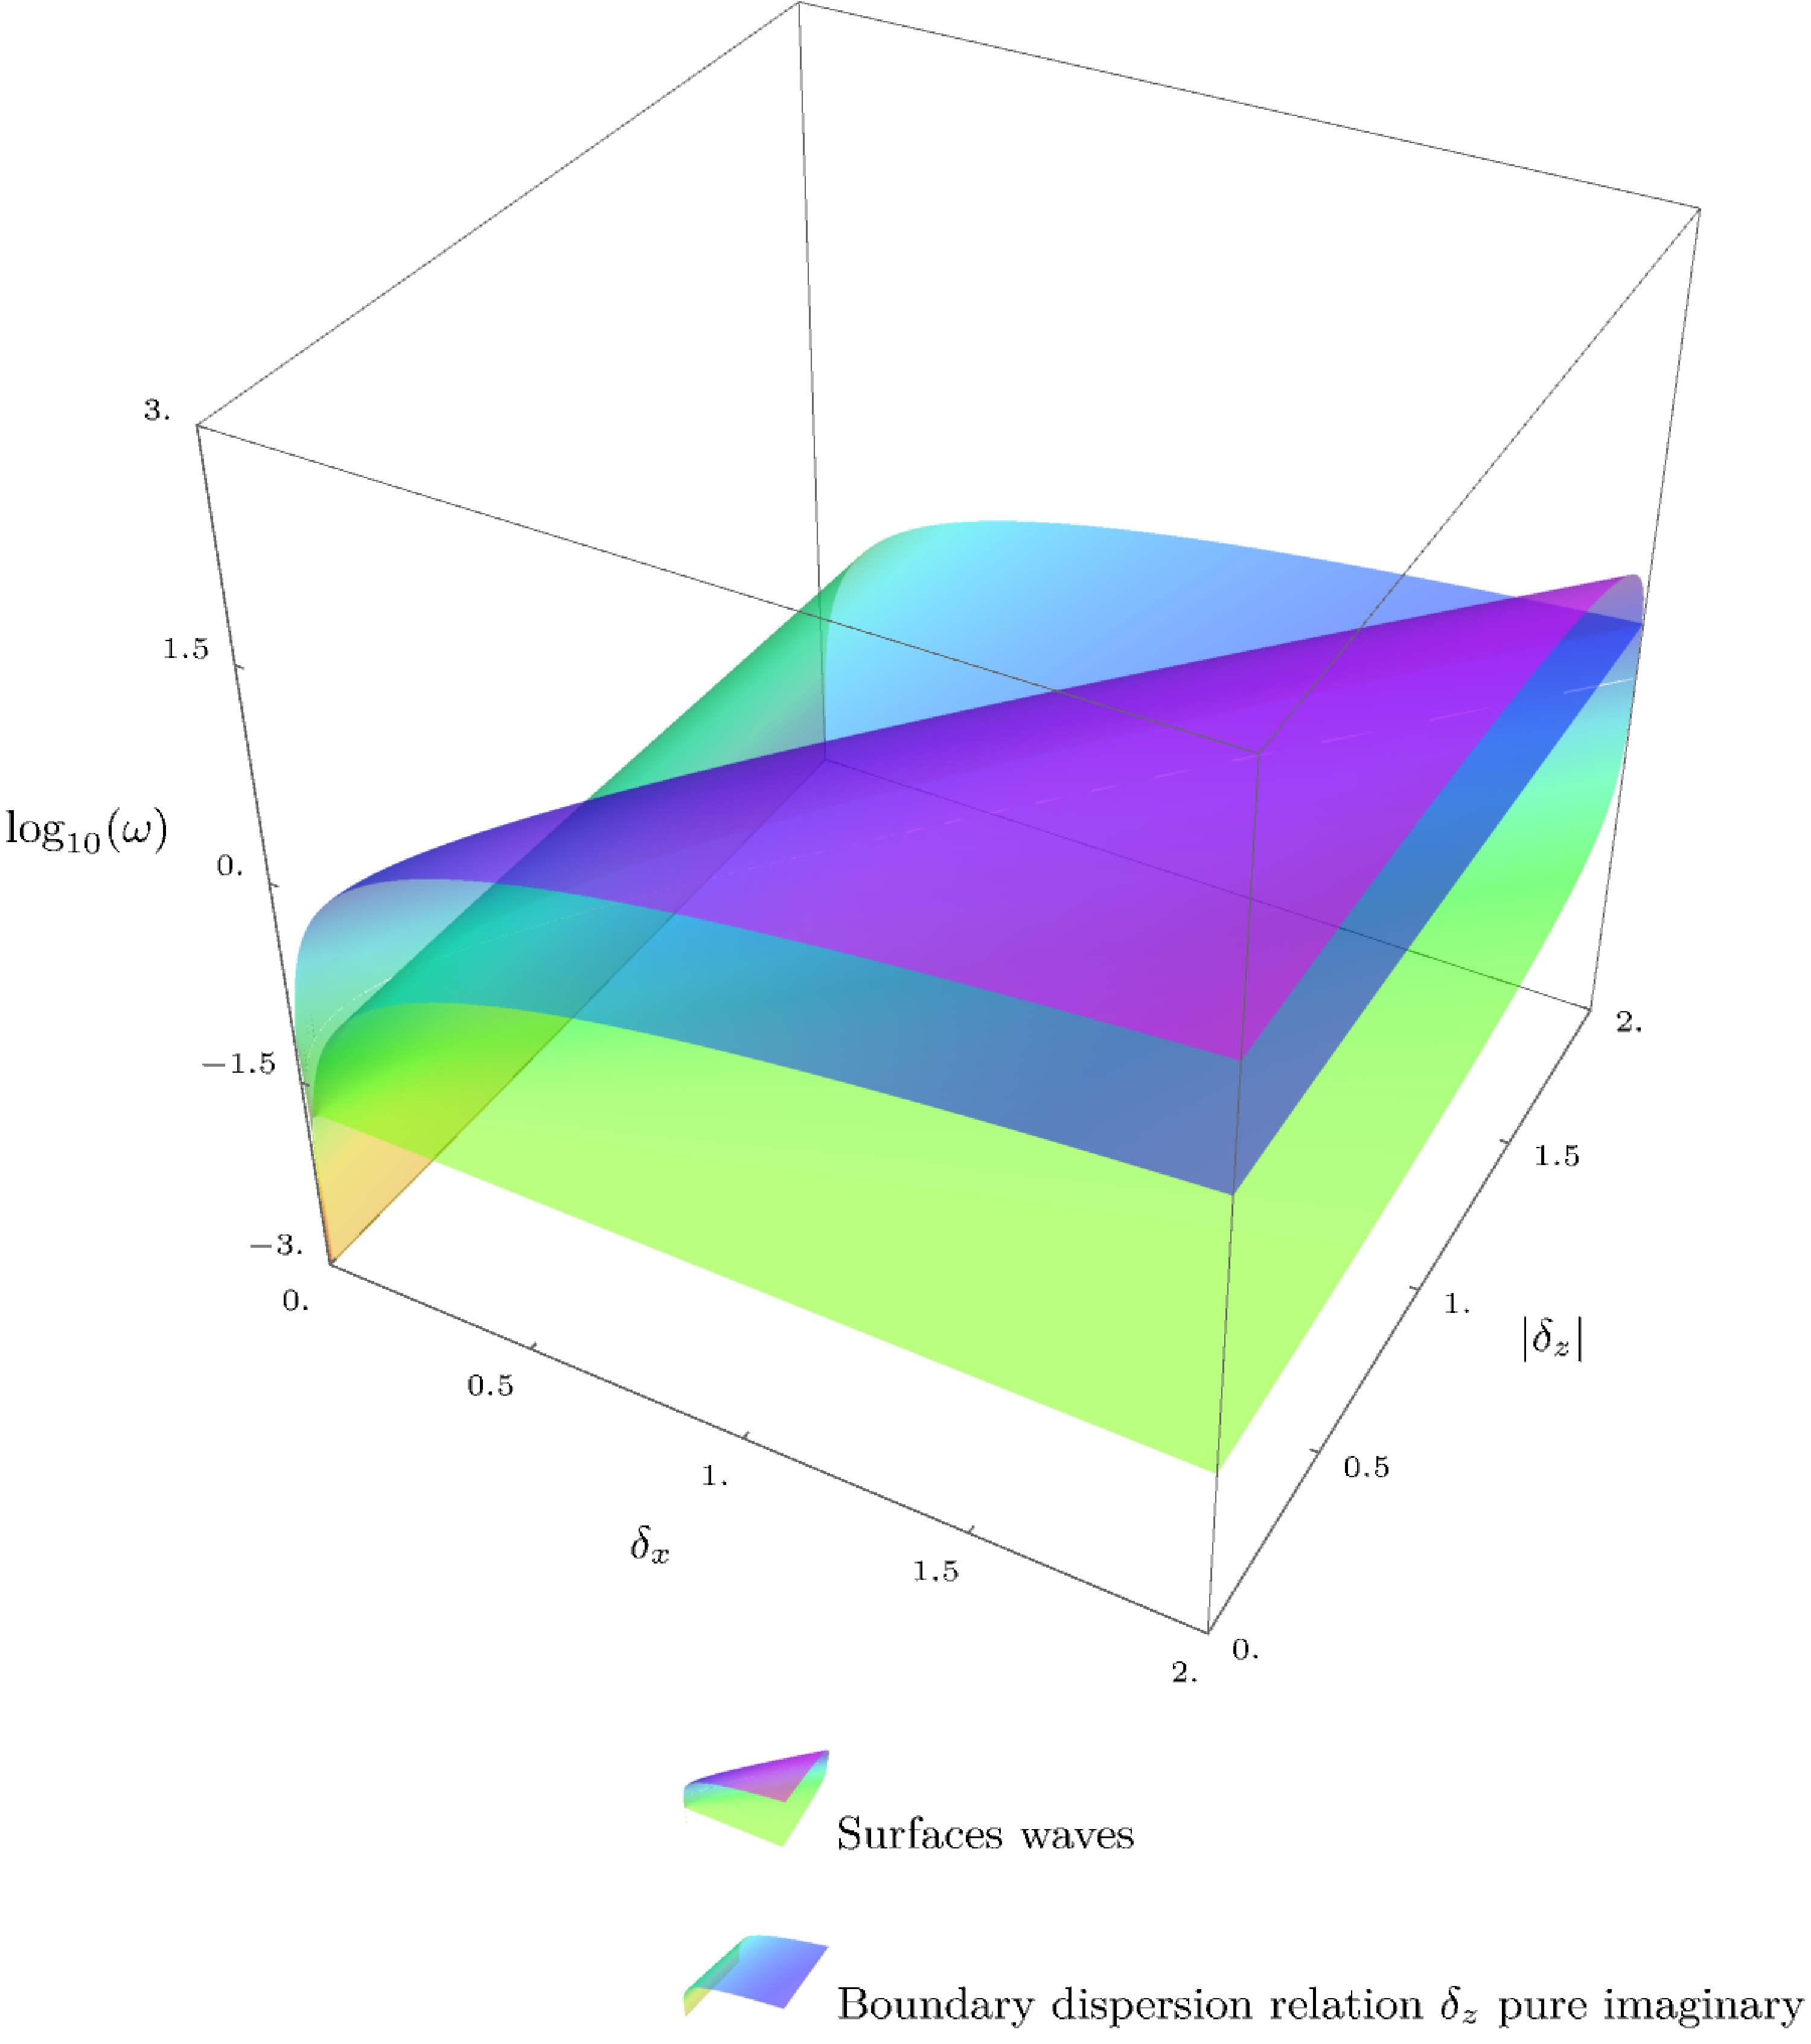
\includegraphics[width=0.45\linewidth]{FIGURES/boundedimaginary.png}
}
	\caption{\textit{Dispersion surfaces in $(\delta_x,\ \delta_z,\log_{10}(\omega))$  space and wave solutions.\\
	%	Wave solutions. Polychrome surfaces: Inner dispersion surface for real $\delta_z$ (acoustic and gravity branches). Blue: Boundary dispersion surface. Black points: acoustic wave (upper branch) and internal wave solutions (lower branch).
		%
			 (a) Wave solutions with real $\delta_z$. Polychrome surfaces: inner dispersion surfaces (acoustic and internal branches) and Boundary dispersion surface.\\
			 (b) Wave solutions with purely imaginary $\delta_z$. Polychrome surfaces: inner dispersion surface (surface gravity-wave branch) and Boundary dispersion surface.
		%	 (c) Wave solutions in the vicinity of the origin. Polychrome surface: Lower (respectively upper) $\delta_x$: inner dispersion surface for real $\delta_z$ (pure imaginary $\delta_z$). Blue: Boundary dispersion surface. Black (red) points: surface wave solutions.\\
		%	 (d) Wave solutions with both real and pure-imaginary wave-numbers as given in (a) and (b).
	}
}
\label{FigDispSolutions}
\end{figure}
%\begin{figure}[!h]
%	\centering		
%	\begin{subfigure}{0.45\linewidth}
%		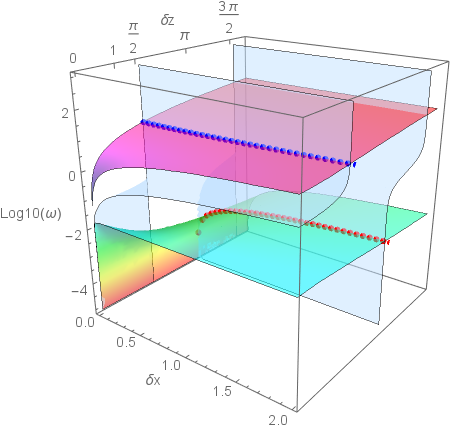
\includegraphics[width=1\linewidth]{FIGURES/Fig_Inter_Real.png}
%		\caption{}
%	\end{subfigure}
%	~
%	\centering
%	\begin{subfigure}{0.45\linewidth}
%		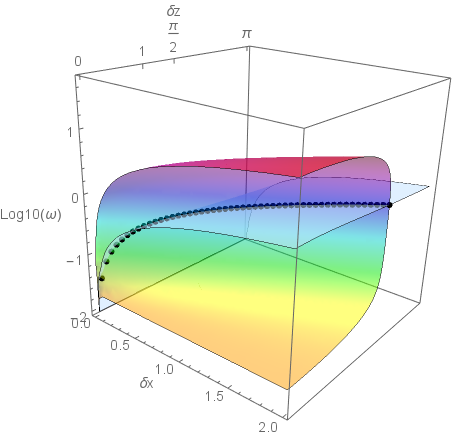
\includegraphics[width=1\linewidth]{FIGURES/Fig_Inter_Imag.png}
%		\caption{}
%	\end{subfigure}
%	
%	\begin{subfigure}{0.45\linewidth}
%		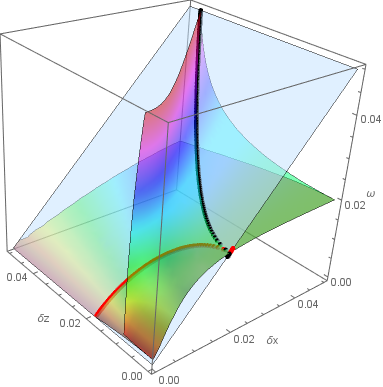
\includegraphics[width=1\linewidth]{FIGURES/Fig_Inter_All_zoom5.png}
%		\caption{}
%	\end{subfigure}
%	~
%	\begin{subfigure}{0.45\linewidth}
%		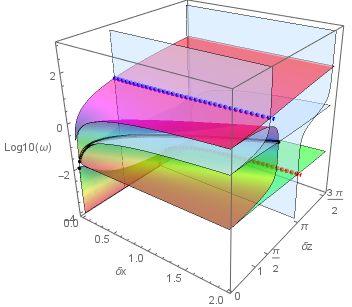
\includegraphics[width=1\linewidth]{FIGURES/Disp_Full_all.png}
%		\caption{}
%	\end{subfigure}
%
%	\caption{\textit{Dispersion surfaces in $(\delta_x,\ \delta_z,\ Log_{10}(\omega)$ or $\omega)$  space and wave solutions.\\
%Wave solutions. Polychrome surfaces: Inner dispersion surface for real $\delta_z$ (acoustic and gravity branches). Blue: Boundary dispersion surface. Black points: acoustic wave (upper branch) and internal wave solutions (lower branch).
%%
%%	 (a) Wave solutions with real $\delta_x$. Polychrome surfaces: Inner dispersion surface for real $\delta_z$ (acoustic and gravity branches). Blue: Boundary dispersion surface. Black points: acoustic wave (upper branch) and internal wave solutions (lower branch).\\
%%	 (b) Wave solutions with pure imaginary $\delta_x$. Polychrome surface: Inner dispersion surface for pure imaginary $\delta_z$ (surface gravity-wave branch). Blue: Boundary dispersion surface. Red points: surface wave solutions.\\ 
%%	 (c) Wave solutions in the vicinity of the origin. Polychrome surface: Lower (respectively upper) $\delta_x$: inner dispersion surface for real $\delta_z$ (pure imaginary $\delta_z$). Blue: Boundary dispersion surface. Black (red) points: surface wave solutions.\\
%%	 (d) Wave solutions with both real and pure-imaginary wave-numbers as given in (a) and (b).
% }
% }
%	\label{FigDispSolutionsold}
%\end{figure}
%For pure-imaginary vertical wave numbers, the inner dispersion surface is folded both for large and small pulsations. For real vertical wave-numbers branches are present in the upper and lower regions as could be expected by adding the transformations already observed in figure \ref{FigFullHomogeneous} when $\epsilon_i$ and $\epsilon_a$ were separately non zero. In the large-pulsation region, the upper branch of the inner dispersion surface is similar to figure (\oldref{FigFullHomogeneous}.c) and, once again, could not be distinguished from the $\omega^2=\omega_a^2$ surface. The same is true in the small-pulsation region where the lower branch of the inner dispersion surface could this time not be distinguished from the $\omega^2=\omega_i^2$ surface. This is a consequence of the separation of the roots of the inner dispersion relation \ref{solseq} or equivalently of the separation of the upper, acoustic and lower, acoustic branches already observed in figure \ref{FigFullHomogeneous}: when $\epsilon_i$ and $\epsilon_a$ are simultaneously non zero, MAW and MIW can simultaneously propagate. Nevertheless, relations \ref{DispAcousDT} and \ref{DispRaysDT} show that at higher order in this small parameters, their dispersion relations are modified by the stratification and/or the compressibility of the ocean. Figure \oldref{FigDispSolutions}.d additionally provides all dispersion surface branches on the same plot. It confirms inequality \ref{RelInequal}. The inner-dispersion surface for pure-imaginary wave-numbers is bounded by the same surfaces for real wave-numbers.\\
For real vertical wavenumbers ($k_z\in\mathbb{R}$, Figure \oldref{FigDispSolutions}a), the boundary dispersion surface is a piecewise surface. It includes several branches that are vertical (in the $(\delta_x, \delta_z, \log_{10}(\omega)$) space) at $\delta_z \approx n\pi$ (small values of $\omega$) and at $\delta_z \approx \pi/2+m\pi$ (large values of $\omega$), with $n\in\mathbb{N}^\ast$ and $m\in\mathbb{N}$. The intersection of these branches with the inner dispersion relation surfaces result in a number of constrained vertical wavenumbers (according to the values of $n$ and $m$), the resulting wave solutions will thus be called {\it modes}. The two intersections correspond to {\it Modified Internal Modes (MIM),  $n\in\mathbb{N}^\ast$} and to {\it Modified Acoustic Modes (MAM), $m\in\mathbb{N}$}.\\
For purely imaginary wavenumbers (Eq. \ref{EqFullDisperbi}), the boundary surface (Figure \oldref{FigDispSolutions}b) looks like an horizontal hyperbolic surface which intersects the surface waves surface. Far from the origin $(\delta_x,\delta_z)=(0,0)$, at the intersection points, $|\delta_z|$ is close to $\delta_x$.
%\textit{Numerical approximations of wave solutions in a bounded ocean:}\\
%Figure \ref{FigDispSolutions} confirms for this model of compressible, stratified, free-surface ocean, the existing of three types of intersections between the inner and boundary dispersion surfaces and, as a consequence, three regions of phase-space where waves can propagate in a bounded ocean. These intersections are shown by three lines of color points. The black-point intersection corresponds to wave-solutions propagating with a pure imaginary vertical wave-number in the middle-range pulsation region (figures \oldref{FigDispSolutions}.b, c and d). These are surface (edge) vertically-vanishing waves propagating in a compressible, stratified ocean, hereafter named Modified Surface Waves (MSW). Figure \oldref{FigDispSolutions}.d shows that they occupy a region of phase-space where the inner dispersion surface is approximately vertical and tangent to the $\delta_x\approx\delta_{z,i}$ plane meaning that the influence of compressibility and stratification (gravity) are both small. 
%
%The red and blue lines of points indicate that two remaining wave-solutions are possible, this time with real vertical wave-numbers. One (blue points) is an intersection of the boundary dispersion surface with the upper acoustic branch of the inner dispersion surface (figures \oldref{FigDispSolutions}.a, c and d), the other (red points) is an intersection of the same boundary dispersion surface with the lower stratification branch of the inner dispersion surface (figures \oldref{FigDispSolutions}.a and d). Since in both cases, vertical wave-numbers are quantified ($\delta_z = \pi/2+m\pi$ and $\delta_z \approx n\pi$), the resulting wave solutions can be associated to respectively Modified Acoustic Modes (MAM) and Modified Internal Modes (MIM), these modes being modified by both compressibility and stratification (gravity).\\
\paragraph{Long-wave solutions}
For long waves ($|\delta_z| \ll 1$), the boundary dispersion surfaces for real and purely imaginary $\delta_z$ coincide. Indeed the development of the boundary relation is well approximated by $\omega^2\approx \delta_x^2$ in both cases (a better approximation is given in Eq. \ref{eqomegalongwavereal}).
Figure \oldref{FigDisLongpSolutions} shows the different branches close to the origin $(\delta_x, \delta_z)=(0,0)$. The acoustic waves surface is not shown since it does not intersect the boundary dispersion surface near the origin (as proved in \S\oldref{SubSectionLongWavesrealdz}).
\begin{figure}[!h]
	\centering		
	%	\begin{subfigure}{0.45\linewidth}
	%		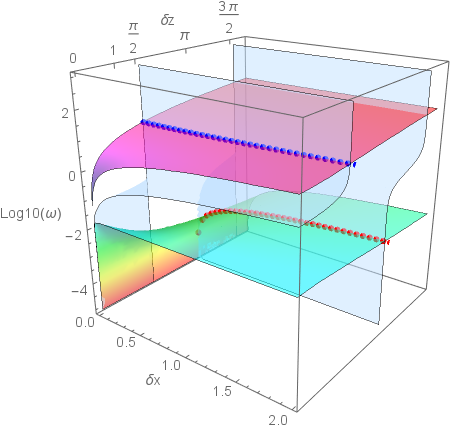
\includegraphics[width=1\linewidth]{FIGURES/Fig_Inter_Real.png}
	%		\caption{}
	%	\end{subfigure}
	%	~
	%	\centering
	%	\begin{subfigure}{0.45\linewidth}
	%		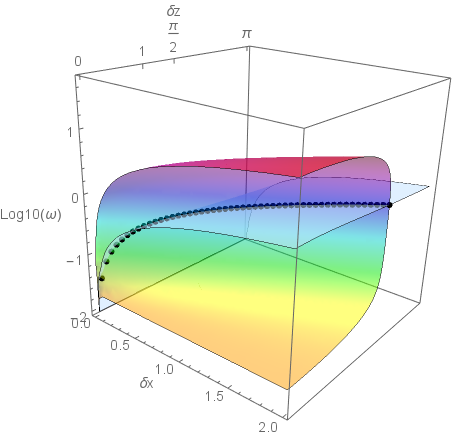
\includegraphics[width=1\linewidth]{FIGURES/Fig_Inter_Imag.png}
	%		\caption{}
	%	\end{subfigure}
	%	
	%	\begin{subfigure}{0.45\linewidth}
		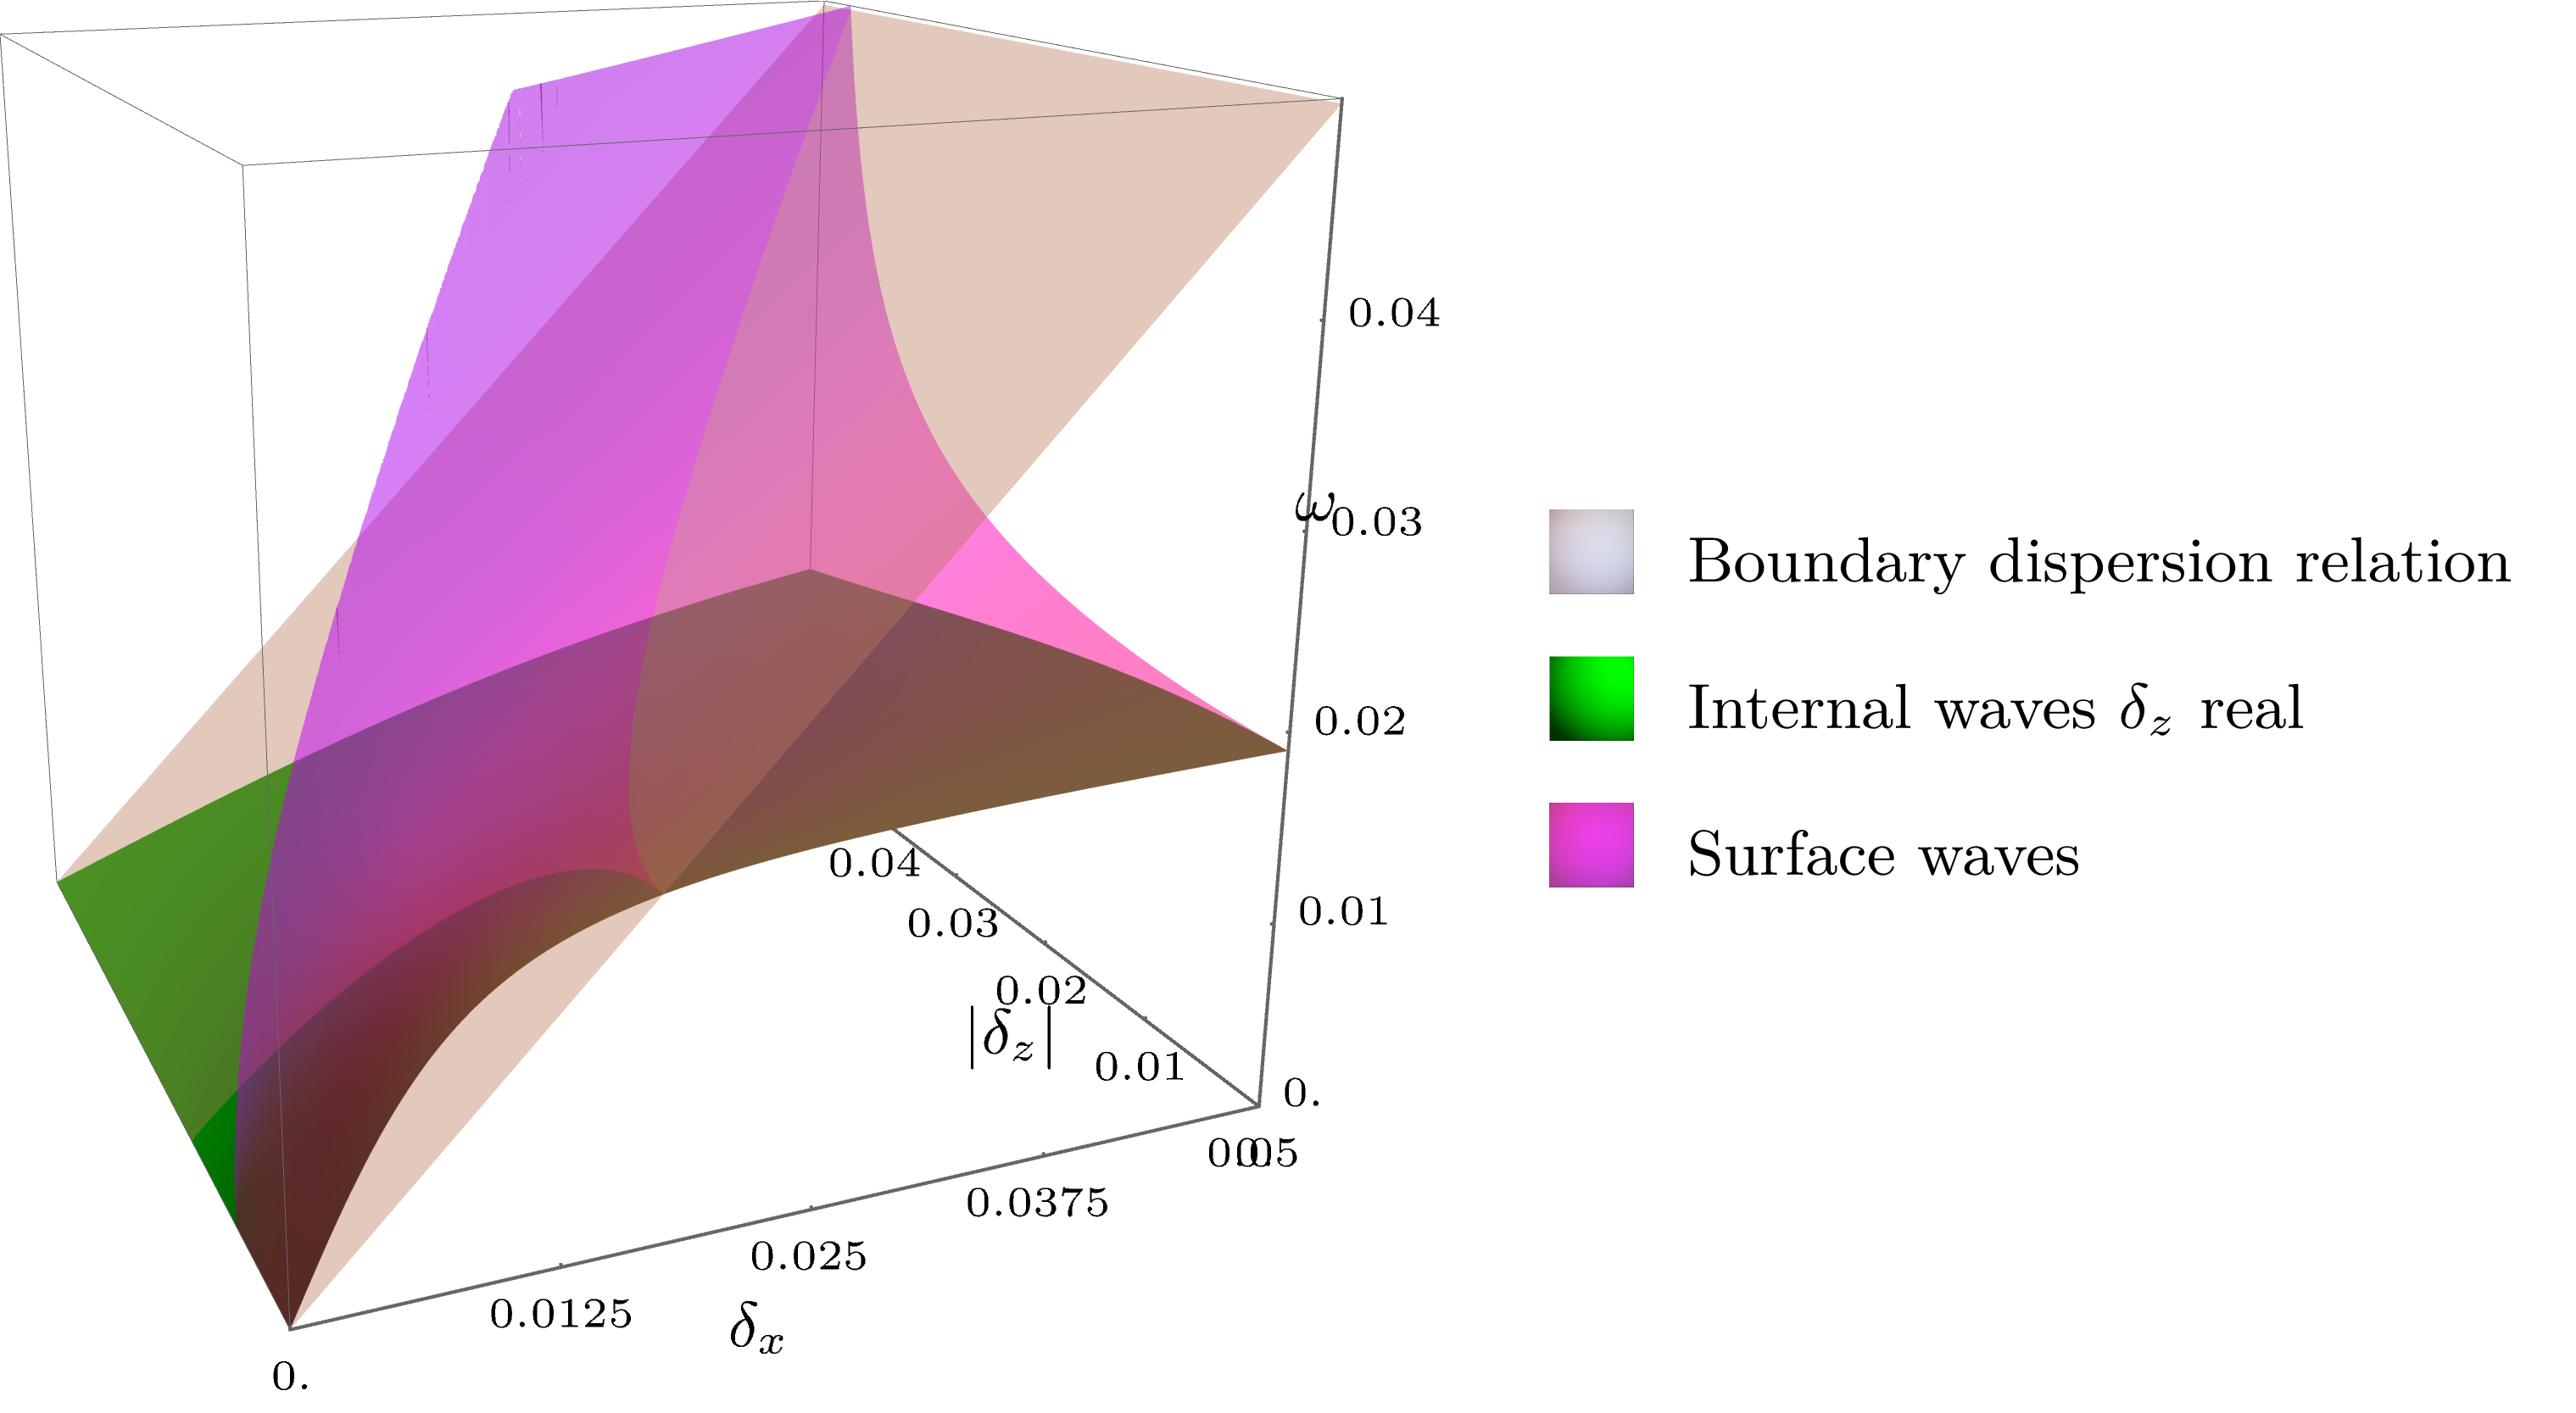
\includegraphics[width=0.6\linewidth]{FIGURES/boundedorigin.png}
	%		\caption{}
	%	\end{subfigure}
	~
	%	\begin{subfigure}{1.\linewidth}
	%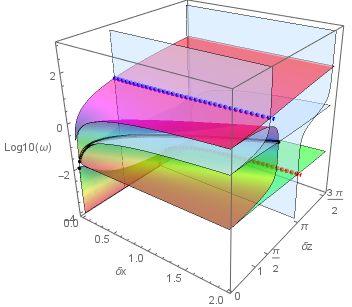
\includegraphics[width=1\linewidth]{FIGURES/Disp_Full_all.png}
	%		\caption{}
	%	\end{subfigure}
	
	\caption{\textit{Dispersion surfaces in $(\delta_x, \delta_z, \omega$) space and wave solutions in the vicinity of the origin. Polychrome surfaces: inner dispersion surfaces (internal and surface branches) and Boundary dispersion surface.
		}
	}
	\label{FigDisLongpSolutions}
\end{figure}
While for very small values of $\delta_x$, the boundary dispersion surface intersects the internal waves branch (with $\delta_z$ real), for larger values, it intersects the surface waves branch (with $\delta_z$ pure imaginary). As will be shown in section \oldref{SubSectionLongWavesrealdz}, the switch between the two intersections is at a value of $\delta_x=\delta_{x,0}\approx \epsilon_i$ (and for a vanishing vertical wavenumber $\delta_z=0$).
%In this figure \oldref{FigDisLongpSolutions}, the black-point intersection is the continuation for small wave-numbers of the MSW intersection in Figure \oldref{FigDispSolutions}b whereas the red-point intersection is not connected to the MIM intersection shown in Figure \oldref{FigDispSolutions}a. This continuous-by-part intersection leads to wave-solutions whatever $\delta_x$ in this region. For small values of $\delta_x$ the solution is given by the MIM branch (red points) whereas for larger values of $\delta_x$ it is given by the MSW branch (black points) and the vertical wavenumber vanishes in between these solutions.
\\
{\color{red}remarque ci-dessous: je vous laisse rephraser ... Duko dit (comme nous en fait) que la frequence du mode barotrope sature à $\epsilon_i$. (la phrase ci-dessous laisse penser qu'on est pas d'accord avec ca). Par contre, l'ami Duko a l'air de dire (cf Fig9.) que ce mode barotrope existe même pour des valeurs "grandes" de $\delta_x$ (ce qui parait complètement débile, puisque dans ce cas, elles sont où les ondes de surface non hydro classiques ?, quel gros naze ce Duko), alors que nous on montre que c'est seulement pour $\delta_x\le \epsilon_i$ et qu'ensuite ça passe dans la branche ondes de surface (et bien sûr on n'aurait eu que cette branche si on était partis des eqns.  Boussinesq, incompressible, comme dans les "Textbooks") cites par Dukowicz.}
Interestingly,  and contrary to conclusions in \cite{dukowicz_2013}, the barotropic mode pulsation cannot saturate at the buoyancy pulsation for increasing horizontal wavenumber $\delta_x$ but transforms into a vertically evanescent surface wave, while its vertical number switches from real to purely imaginary.
\paragraph{Summary}
In the context of a bounded ocean, three types of wave solutions spreading on the three branches of the inner dispersion surface have thus been identified graphically: internal gravity (in a stratified ocean), acoustic (in a compressible ocean) and surface waves (in a free-surface ocean) and satisfying at the same time the boundary dispersion relation. They will be investigated in the next subsections, where analytical expressions are systematically derived using Taylor expansions of the general roots $\omega_{\pm}$ with respect to small parameters $(\epsilon_i,\ \epsilon_a)$, leading to simple approximations of wave dispersion relations. When necessary, asymptotic relations are derived with respect to $\delta_x$, $\delta_z$ or $\omega$. The Taylor expansions additionally give indications on how usual wave solutions can be modified by gravity and stratification $(\epsilon_i)$, and/or by compressibility $(\epsilon_a)$.
%%%%%%%%%%%%%%%%%%%%%%%%%%%%%%%%%%%%%%%%%%%%%%%%%%%%%%%%%%%%%%%%%%%%%%%%%%%%%
\subsection{Real $\delta_z$: modified internal and acoustic waves}
As shown in \S\oldref{realwavenumber}, as long as $\delta_z$ is not close to zero, the upper (acoustic) and lower (gravity) branches of the inner dispersion surface for real $\delta_z$ are well-separated and the MAM and MIM solutions can thus be studied independently for real vertical wavenumbers. The case of long waves with $\delta_z \approx 0$ is discussed in subsection \oldref{SubSectionLongWavesrealdz}.
%
\subsubsection{Development of internal-gravity modes modified by compressibility (MIM)}
\label{SubSectionGraphicMIW}
%%%%%%%%%%%%%%%%%%%%%%%%%%%%%%%%%%%%%%%%%%%%%%%%%%%%%%%%%%%%%%%%%%%%%%%%%%%%%
%The mode-0 (barotropic) MIM solution will be investigated in section \ref{SubSectionGraphicMSW} and, as a consequence, only solutions for not small vertical wave-numbers needs to be explored here.
Waves can propagate horizontally between the bottom and surface of the ocean as in a wave guide. Internal gravity modes are  well-known such examples \citep{gill_1982}. In the previous section, graphical inspections of wave solutions confirmed that gravity waves with constrained vertical wavenumbers could be found at the intersection of the inner and boundary dispersion surfaces.
We have also shown in \S\oldref{realwavenumber} that the root of the inner dispersion relation corresponding to internal gravity waves is well-approximated by $\omega_i^2$. Making $\omega^2(\delta_x) \approx\omega_i^2$ in the boundary dispersion relation \ref{EqFullDisperb} leads to 
%\[
%	   \label{DispSysIntModesab}
%	\omega^2(\delta_x) \approx\omega_i^2\implies	\frac{\delta_x^2}
	%	{\delta_z/\tan(\delta_z)+\frac{\epsilon_i^2+\epsilon_a^2}{2}}	\approx
	%	\frac{\epsilon_i^2 \delta_x^2}{\delta_x^2
	%	+\delta_z^2+\frac{1}{4}\left(
	%	\epsilon_i^2+\epsilon_a^2\right)^2}
%\]
%
\begin{equation}
		\frac{1}
{\delta_z/\tan(\delta_z)+\frac{\epsilon_i^2+\epsilon_a^2}{2}}
\approx
\frac{\epsilon_i^2}{\delta_x^2
	+\delta_z^2+\frac{1}{4}\left(
	\epsilon_i^2+\epsilon_a^2\right)^2}
\label{equimim}
\end{equation}
Since we have assumed here that $\delta_z$ is not close to 0, the right-hand side of \ref{equimim} is always small and thus $\delta_z/\tan(\delta_z)$ has to be large: the vertical wavenumber $\delta_z$ has to be close to $n\pi$ with $n$ a non-zero integer. This agrees with the internal gravity wave solution found graphically in subsection \oldref{SubSectionPotBranches}.\\
In order to get a more precise approximation, we equate the squared frequency given by the surface dispersion relation \ref{EqFullDisperb} to $\omega_-^2$ the one given by the inner dispersion relation \ref{solseq}. This forms a non-linear equation for $\delta_z$ whose solution is then approximated using two passes of a Newton algorithm starting from $\delta_z=\delta_{z,n}$. Finally a Taylor development in term of $\epsilon_i, \epsilon_a$ is performed to get:
\begin{equation}
\delta_{z}(\delta_x)=\delta_{z,mim}(\delta_x)=
	\delta_{z,n}
	\left(
	1+\frac{\epsilon_i^2}{\delta_x^2+\delta_{z,n}^2}
	+\frac{(\delta_x^2-\delta_{z,n}^2)}{(\delta_x^2+\delta_{z,n}^2)^3}\epsilon_i^4
	\right)
	+\mathrm{O}	((\epsilon_i^2+\epsilon_a^2)^3)
	\label{ParamallMIM1}
\end{equation}
\nhi{idem 'ordre 2 inclus}
\hi{
\begin{equation}
\delta_{z}(\delta_x)=\delta_{z,mim}(\delta_x)=
\delta_{z,n}
\left(
1+\frac{\epsilon_i^2}{\delta_{z,n}^2}
-\frac{1}{(\delta_{z,n}^4)}\epsilon_i^4
\right)
+\mathrm{O}	(\epsilon_i^6)
\end{equation}
}
A development for the frequency $\omega^2$ can be obtained by injecting the expression of $\delta_z$ given by \ref{ParamallMIM1} in the general expression \ref{DispRaysDT} in the unbounded domain case.\\
The usual dispersion relation given in Table \oldref{TableWave solutions} would write in dimension form:
\[
\omega^2=\left.\omega_{iwr}^2\right|_{\delta_z=\delta_{z,n}}=\epsilon_i^2\frac{\delta_x^2}{\delta_x^2+\delta_{z,n}^2}
\]
If we are concerned more specifically with the main distinction (i.e. first order correction) to this relation, we omit all the terms of order 3 in $(\epsilon_i^2+\epsilon_a^2)$ in \ref{DispRaysDT} to get:
 \begin{equation}
\omega^2(\delta_x)=\omega_{mim}^2(\delta_x)=
\epsilon_i^2\frac{\delta_x^2}{\delta_x^2+\delta_{z,n}^2}
\left(1-\frac{2\epsilon_i^2\delta_{z,n}^2}{(\delta_x^2+\delta_{z,n}^2)^2}\right) +\mathrm{O}	((\epsilon_i^2+\epsilon_a^2)^3)
\label{ParamallMIM2}
\end{equation}
\nhi{idem 'ordre 2 inclus}
\hi{
	\begin{equation}
\omega^2(\delta_x)=\omega_{mim}^2(\delta_x)=
\epsilon_i^2\frac{\delta_x^2}{\delta_{z,n}^2}
\left(1-\frac{2\epsilon_i^2}{\delta_{z,n}^2}\right) +\mathrm{O}	(\epsilon_i^6)
	\end{equation}
}
And so the main correction to the usual dispersion relation comes from the fact that $\delta_z$ is not exactly equal to $\delta_{z,n}=n\pi$.
%This shows that the internal gravity modes are robust to compressibility since there is no dependency to $\epsilon_a$ at orders lower than 4. This agrees with the separation of the roots $\omega_\pm$ of the inner dispersion relation for real vertical wave-numbers.
%\\
%A simpler parametric relation can further be found in the vicinity of $\delta_{z,n}^0$ in the long-wave limit using a Taylor development for vanishing $\delta_x$, $\epsilon_i$ and $\epsilon_a$:
%\begin{subequations}
%	   \label{EqParamInt}
%	\begin{alignat}{2}	
%	   \label{ParamMIM1}
%	   %
%		& \delta_z(\delta_x)=\delta_{z,lmim\pi}(\delta_x) &&= 
%		\delta_{z,n}^0+\frac{\epsilon_i^2}{\delta_{z,n}^0} \left(
%		1-\frac{\delta_x^2}{(\delta_{z,n}^0)^2} \right)
%		+\mathrm{O}	(\delta_x^4,\epsilon_i^4,\epsilon_a^4)\\[3mm]
%		%
%	   \label{ParamMIM2}
%		& \omega(\delta_x)=\omega_{lmim\pi}(\delta_x) &&=\epsilon_i\frac{\delta_x}{\delta_{z,n}^0} 
%		\left( 1
%		-\frac{\delta_x^2}{2(\delta_{z,n}^0)^2} \right)
%		+\mathrm{O}	(\delta_x^5,\epsilon_i^3,\epsilon_a^3)
%	\end{alignat}
%\end{subequations}
%For a vanishing horizontal wave-number, these parametric relations show that the pulsation vanishes too but the vertical wave-number is not exactly equal to $\delta_{z,n}^0$ and $\delta_z$ varies with the square of the stratification parameter $(\epsilon_i)$.\\
%This approximate solution is plotted in figure (\oldref{Fig_Approx}.b) (red dash-dotted line) together with the MIM approximation $(\ \delta_{z,mim}(\delta_x),\ \omega_{mim}(\delta_x)\ )$ (red dashed line). The latter MIM approximation cannot be distinguished from the numerical solution.

%
%%%%%%%%%%%%%%%%%%%%%%%%%%%%%%%%%%%%%%%%%%%%%%%%%%%%%%%%%%%%%%%%%%%%%%%%%%%%%
\subsubsection{Development of acoustic Modes modified by gravity (MAM)}
\label{SubSectionGraphicMAW}
%%%%%%%%%%%%%%%%%%%%%%%%%%%%%%%%%%%%%%%%%%%%%%%%%%%%%%%%%%%%%%%%%%%%%%%%%%%%%
%\subsection{Compressible zero-gravity ocean}
%In the particular case of zero-gravity ocean ($\epsilon_i = 0$), the dispersion relations %(\ref{EqFullDisper}) simplify to:

%\begin{subequations}
%	\begin{alignat}{2}	
 %		& \delta_x^2+\delta_z^2 &&=\epsilon_a^2 (\omega^2-\frac{1}{4})\\
%		& \omega^2 &&=\frac{\delta_x^2\ tan(\delta_z)}
%		{\delta_z+\frac{\epsilon_a^2}			{2}tan(\delta_z)}
%		=\frac{\delta_x^2}{\frac{\epsilon_a^2}{2}+\delta_z cotan(\delta_z)}
%	\end{alignat}
%\end{subequations}
Here we use the fact that the root of the inner dispersion relation corresponding to internal gravity waves is well-approximated by $\omega_a^2$. Making $\omega^2(\delta_x) \approx\omega_a^2$ in the boundary dispersion relation \ref{EqFullDisperb} leads to 
%\[
%1/\omega^2(\delta_x) \approx 1/\omega_a^2\implies
%\frac{\delta_z/\tan(\delta_z)+\frac{\epsilon_i^2+\epsilon_a^2}{2}}
%{\delta_x^2}
%\approx
%\frac{\epsilon_a^2}{\delta_x^2
%	+\delta_z^2+\frac{1}{4}\left(
%	\epsilon_i^2+\epsilon_a^2\right)^2}
%=\frac{\delta_x^2\tan(\delta_z)}
%{\delta_z+\frac{\epsilon_i^2+\epsilon_a^2}{2}\tan(\delta_z)}
%\]
%or
\begin{equation}
\label{DispSysIntModesab}
\delta_z/\tan(\delta_z)+\frac{\epsilon_i^2+\epsilon_a^2}{2}
\approx
\frac{\epsilon_a^2}{1
	+\left(\delta_z^2+\frac{1}{4}\left(
	\epsilon_i^2+\epsilon_a^2\right)^2\right)/\delta_x^2}
%=\frac{\delta_x^2\tan(\delta_z)}
%{\delta_z+\frac{\epsilon_i^2+\epsilon_a^2}{2}\tan(\delta_z)}
\end{equation}
Since the right-hand side of \ref{DispSysIntModesab} is small (bounded by $\epsilon_a^2$), $\delta_z/\tan(\delta_z)$ has to be small and thus the vertical wavenumber $\delta_z$ has to be close to $\pi/2+m\pi$, with $m\in\mathbb{N}$.\\
%
Again, in order to get a more accurate expression of $\delta_z$, we equate the (inverse of) squared frequency given by the surface dispersion relation \ref{EqFullDisperb} to the (inverse of) $\omega_-^2$, the frequency given by the inner dispersion relation \ref{solseq} and perform the nonlinear equation's solution approximation followed by a Taylor development in $\epsilon_i, \epsilon_a$ to obtain:
\begin{equation}
	\label{ParamallMAM1}
\begin{array}{l}
\displaystyle
\delta_{z}(\delta_x)=\delta_{z,mam}(\delta_x)=
\delta_{z,m}
-\frac{(\delta_x^2-\delta_{z,m}^2)}{2\delta_{z,m}(\delta_x^2+\delta_{z,m}^2)}\epsilon_a^2
+\frac{\epsilon_i^2}{
2\delta_{z,m}^2}
\\[5mm]
\hspace*{1cm}
\displaystyle
\underbrace{
-\frac{\delta_x^6(\epsilon_a^2-\epsilon_i^2)^2+3\delta_x^2(\epsilon_a^2-\epsilon_i^2)^2\delta_{z,m}^2-\delta_x^2(5\epsilon_a^2-3\epsilon_i^2)(\epsilon_a^2+\epsilon_i^2)\delta_{z,m}^4+(\epsilon_a^2+\epsilon_i^2)^2\delta_{z,m}^6}{4(\delta_x^2+\delta_{z,m}^2)^3\delta_{z,m}^3}
}_{\mathrm{O}	((\epsilon_i^2+\epsilon_a^2)^2)}
\\[5mm]
\hfill
\displaystyle
+\mathrm{O}	((\epsilon_i^2+\epsilon_a^2)^3)
\end{array}
\end{equation}
An expansion  for the frequency $\omega^2$ can be obtained by injecting the expression of $\delta_z$ given by \ref{ParamallMAM1} in the general expression \ref{DispAcousDT} in the unbounded domain case.
The main distinction to the usual acoustic wave frequency, given in Table \oldref{TableWave solutions} in dimensional form, is given by the second-order development:
\begin{equation}
	\label{ParamallMAM2}
	\omega^2(\delta_x) =\omega_{mam}^2(\delta_x)=
	\frac{1}{\epsilon_a^2}
	\left[	\delta_x^2+\delta_{z,m}^2-\frac{(\delta_x^2-\delta_{z,m}^2)}{(\delta_x^2+\delta_{z,m}^2)}\epsilon_a^2+
	\epsilon_i^2
	\right]
		+\mathrm{O}	((\epsilon_i^2+\epsilon_a^2))
\end{equation}
Here, the stratification has a first-order (in term of $\epsilon_i^2$) contribution to the modification of the homogeneous case's frequency. This first-order modification comes from the first-order modification on the vertical wavenumber itself \ref{ParamallMAM1}. However, it is clear that the associated impact is small since $\epsilon_i^2$ is negligible w.r.t. $\delta_{z,m}^2$ in \ref{ParamallMAM1} and \ref{ParamallMAM2}, because $\delta_{z,m} \ge \pi/2$. A similar conclusion was drawn in \cite{smith_2015}.
%%%%%%%%%%%%%%%%%%%%%%%%%%%%%%%%%%%%%%%%%%%%%%%%%%%%%%%%%%%%%%%%%%%%%%%%%%%%%

%%%%%%%%%%%%%%%%%%%%%%%%%%%%%%%%%%%%%%%%%%%%%%%%%%%%%%%%%%%%%%%%%%%%%%%%%%%%%
\subsection{Purely imaginary $\delta_z$: surface acoustic-gravity waves}
\label{SubSectionGraphicMSW}
%%%%%%%%%%%%%%%%%%%%%%%%%%%%%%%%%%%%%%%%%%%%%%%%%%%%%%%%%%%%%%%%%%%%%%%%%%%%%
%In the present section, these approximations are plotted on figure \ref{Fig_Approx}to be compared with the correction numerical approximation obtained in Section \ref{SectionGraphic}.
"Surface waves" generally refer to wave propagating horizontally as anomalies of the ocean free-surface \citep{gill_1982}. In the vertical direction, these surface wave anomalies are "evanescent" meaning that, with the notation chosen in the present study, the vertical wavenumber $\delta_z$ is a purely imaginary complex number.
%An alternative way to introduce "surface waves" is to introduce them as a limiting case of internal gravity mode (Duckowicz, 2015): they are then referred to as a barotropic mode with mode-number "n = 0" (using the notations of Section \ref{SectionGraphic}).\\
%The numerical investigation of long MSW conducted in the previous subsection indicates that these two characterizations refer to two different wave solutions.\\
A MSW defined by its triplet $(\delta_x,\ \delta_z,\ \omega)$ must satisfy both the inner \ref{EqFullDispera} and boundary \ref{EqFullDisperb} dispersion relations for $\delta_z\ =\ i\ \delta_{z,i}$:
%A consequence is that the dispersion relations of these horizontally propagating waves, should, at least locally in phase space, be advantageously parameterized in the form $(\ \delta_{z,i}(\delta_x),\ \omega(\delta_x)\ )$. As already stated before, such a parametrization is yet difficult to formulate since (i) the inner dispersion relation is fourth order in $\omega$ and (ii) the boundary dispersion relation is transcendental in $\delta_z$. A consequence is that analytically-simple, physically meaningful formulations can only be obtained under (very) restrictive assumptions.\\ 
%A way to circumvent these difficulties is to iteratively approximate and substitute $\delta_z(\delta_x)$ and $\omega(\delta_x)$ using both the inner and boundary dispersion relations.\\
\begin{equation}
\delta_x^2-\delta_{z,i}^2 =\epsilon_i^2\frac{\delta_x^2}
{\omega^2}+\epsilon_a^2\omega^2-\frac{(\epsilon_a^2+\epsilon_i^2)^2}{4} \qquad , \qquad
%\label{eqinternecomplexe}
%\end{equation}
%and the surface boundary relation \ref{EqFullDisperb}:
%\begin{equation}
\omega^2=\frac{\delta_x^2}
{\frac{\delta_{z,i}}{\tanh(\delta_{z,i})}+\frac{\epsilon_a^2+\epsilon_i^2}{2}}
%\label{eqsurfacecomplex}
\label{rappel-eqs-complex}
\end{equation}
In an homogeneous and incompressible ocean ($\epsilon_i=\epsilon_a=0$), we get $\delta_{z,i}=\delta_x$. This relation is often postulated in textbooks to reduce the number of variables. Vertical polarization relations are then functions of $\delta_x$ only \citep{gill_1982} and, as a consequence, the only remaining dispersion relation is the boundary dispersion relation \ref{EqFullDisperb} for purely imaginary vertical wavenumber $(\delta_z=i\delta_x)$, or its approximation  $\omega^2=\delta_x \tanh \delta_x$. In this case, $\delta_{z,i}$ is just the vertical length-scale for wave decrease downward from the surface, and for very long waves ($\delta_x \gg 1$), the surface wave is approximately depth-independent.
%
\paragraph{Surface waves existence} In the more general case (non homogeneous and compressible ocean), it is first necessary to study the existence of solutions to \ref{rappel-eqs-complex}. Let define
$f(\delta_x, \delta_{z,i})$ by:
\[
f(\delta_x, \delta_{z,i})=\delta_x^2-\delta_{z,i}^2-\left(
\epsilon_i^2\frac{\delta_x^2}
{\omega^2}+\epsilon_a^2\omega^2-\frac{(\epsilon_a^2+\epsilon_i^2)^2}{4}
\right),
\qquad \mbox{ with }\omega^2=\frac{\delta_x^2}
{\frac{\delta_{z,i}}{\tanh(\delta_{z,i})}+\frac{\epsilon_a^2+\epsilon_i^2}{2}}
\]
The inner boundary relation translates into $f(\delta_x,\delta_{z,i})=0$. It is easy to check that, for a given $\delta_{z,i}$, $f(\delta_x,\delta_{z,i})$ is an increasing function of $\delta_x$\footnote{This simple demonstration requires the assumption $\epsilon_a^2 \le 2 + \epsilon_i^2$, i.e. the same than the one used in appendix to prove that the imaginary part of $\delta_z^2$ is zero.}. Let $\delta_{x,0}$ corresponds to the value of $\delta_x$ such that $f(\delta_{x,0},\delta_z=0)=0$ (the value of $\delta_{x,0}$ is given in \ref{deltazsurface}, $\delta_{x,0}$ is close to $\epsilon_i$).
In particular we have $f(\delta_x,0)\le f(\delta_{x,0},0)=0$ for $\delta_x \le \delta_{x,0}$. It is also easy to verify that for a given $\delta_x$ such that $\delta_x \le \delta_{x,0}$, the maximum of $f(\delta_x,\delta_z)$ is attained in $\delta_{z,i}=0$. This proves that if $\delta_x < \delta_{x,0}$, $f(\delta_x,\delta_{z,i}) < 0\; \forall \delta_{z,i}$. Thus modified surface waves can only exist under the condition $\delta_x \ge \delta_{x,0}$.
%
\paragraph{Dispersion relation}
%The surface dispersion relation helps us to bound the magnitude of the right-hand side of the inner dispersion relation. Indeed, for $\delta_{z,i}\ge 0$, using, e.g., $\displaystyle \frac{\delta_{z,i}+1}{2}\le \frac{\delta_{z,i}}{\tanh(\delta_{z,i})}\le \delta_{z,i}^2+1$, we get
%\[
%\epsilon_i^2\frac{\delta_x^2}{\omega^2}\le \epsilon_i^2\left(\delta_{z,i}^2+1+\frac{\epsilon_a^2+\epsilon_i^2}{2})\right), \qquad \epsilon_a^2\omega^2 \le 2\epsilon_a^2\delta_x^2
%\]
%and thus we have
%\[
%-\frac{(\epsilon_a^2+\epsilon_i^2)^2}{4}\le \delta_x^2 - \delta_{z,i}^2 \le \epsilon_i^2 \delta_{z,i}^2+2\epsilon_a^2\delta_x^2
%+\epsilon_i^2\left(1+\frac{(\epsilon_a^2+\epsilon_i^2)}{2}\right)
%\]
%
It can be shown that $\displaystyle 1\le \frac{\delta_{z,i}}{\tanh(\delta_{z,i})}\le \delta_{z,i}^2+1, \quad \forall \delta_{z,i}\in\mathbb{R}$. Injecting these two inequalities in the surface dispersion relation directly leads to 
\[
\frac{\delta_x^2}{\omega^2}\le \delta_{z,i}^2+1+\frac{\epsilon_a^2+\epsilon_i^2}{2}, \qquad \hbox{and}\qquad \omega^2 \le \delta_x^2
\]
%
Since  
the inner dispersion relation  implies 
$\displaystyle
-\frac{(\epsilon_a^2+\epsilon_i^2)^2}{4}\le \delta_x^2 - \delta_{z,i}^2 
\le \epsilon_i^2\frac{\delta_x^2}
{\omega^2}+\epsilon_a^2\omega^2$, we finally get
%
\[
-\frac{(\epsilon_a^2+\epsilon_i^2)^2}{4}\le \delta_x^2 - \delta_{z,i}^2 
\le \epsilon_i^2 \delta_{z,i}^2+\epsilon_a^2\delta_x^2
+\epsilon_i^2\left(1+\frac{\epsilon_a^2+\epsilon_i^2}{2}\right)
\]
%
Using the smallness of the parameters $\epsilon_a$ and $\epsilon_i$, we can then conclude that $\delta_{z,i}^2$ is indeed close to $\delta_x^2$. 
\par
%
The crude  assumption $\delta_{z,i} \approx \delta_x$ is sufficiently accurate to recover usual swell-like approximations (Table \oldref{TableWave solutions}), i.e. for sufficiently large $\delta_x$ (or $\delta_z$). However a more accurate expression is given by
\begin{equation}
\delta_{z,i}^2=\delta_x^2
-\delta_x\left(
\epsilon_i^2/\tanh(\delta_x)+\epsilon_a^2\tanh(\delta_x)
\right)
+\mathrm{O}	((\epsilon_i^2+\epsilon_a^2)^2).
\label{longMSW}
\end{equation}

\nhi{
\begin{equation}
\delta_{z,i}^2=\delta_x^2
-\delta_x\left(
\epsilon_i^2/\tanh(\delta_x)
\right)
+\mathrm{O}	(\epsilon_i^4).
\end{equation}
}
\hi{
No solution
}
In order to obtain \ref{longMSW}, we introduce the frequency given by the boundary dispersion relation in the inner dispersion relation (see \ref{rappel-eqs-complex}) and solve the resulting nonlinear equation by performing one pass of a Newton algorithm. Note that the problem is formulated in term of $\delta_{z,i}^2(\delta_x)$ since it can be shown (by looking at the error estimate of the Newton algorithm) that a formulation in term of $\delta_{z,i}(\delta_x)$ is not accurate when $\delta_x$ is relatively small.
Note that expression \ref{longMSW} requires $\delta_x \ge \epsilon_i$ for $\delta_{z,i}^2$ to be positive. This is consistent with the fact that $\delta_x$ has to be greater than $\delta_{x,0} (\approx \epsilon_i)$, which has been shown previously. However expression \ref{longMSW} does not allow to recover this exact value $\delta_{x,0}$ of $\delta_x$ that cancels $\delta_{z,i}$, due to the first-order only approximation in term of $(\epsilon_i^2+\epsilon_a^2)$. The case of long surface waves with $\delta_{z,i}$ close to zero will be treated separately in  subsection \oldref{SubSectionLongWavesrealdz}.
\\
The corresponding frequency is well approximated by
\begin{equation}
\omega^2=\delta_x \tanh(\delta_x)
\left[1-\frac{1}{2}\left(
\epsilon_i^2/\sinh(\delta_x)^2+\epsilon_a^2/\cosh(\delta_x)^2-\epsilon_i^2/(\delta_x\sinh(\delta_x)\cosh(\delta_x)
\right)
\right]+\mathrm{O}	((\epsilon_i^2+\epsilon_a^2)^2)
\label{eqomegasurfacewaves}
\end{equation}
\nhi{
	\begin{equation}
	\omega^2=\delta_x \tanh(\delta_x)
	\left[1-\frac{1}{2}\left(
	\epsilon_i^2/\sinh(\delta_x)^2-\epsilon_i^2/(\delta_x\sinh(\delta_x)\cosh(\delta_x)
	\right)
	\right]+\mathrm{O}	(\epsilon_i^4)
	\end{equation}
}
\hi{
	No solution
}
%
For very short waves ($\delta_x \gg 1$), these relations simplify to:
\[
\delta_{z,i}\approx \delta_x
-\frac{1}{2}\left(
\epsilon_i^2+\epsilon_a^2
\right)
,\quad
\omega^2\approx \delta_x
\]
\nhi{
	\[
	\delta_{z,i}\approx \delta_x
	-\frac{1}{2}\left(
	\epsilon_i^2
	\right)
	,\quad
	\omega^2\approx \delta_x
	\]
}
\hi{
	No solution
}
and we recover the frequency of short non hydrostatic waves $\omega^2 = \delta_x$ (or $\Omega=\sqrt{gk_x}$ in dimensional form) with a slightly modified vertical wavenumber.
%
%
\subsection{Long waves}
\label{SubSectionLongWavesrealdz}
We here perform specific developments for long waves where the vertical profile is almost depth-independent $\delta_z \approx 0$, $\delta_z$ being either real or purely imaginary.
Inserting the boundary dispersion relation \ref{EqFullDisperb} into the inner dispersion relation \ref{EqFullDispera} and making a second-order Taylor expansion in $\delta_z$ leads to:
\begin{equation}
	\delta_z^2=\left(
	\delta_{x,0}^2-\delta_x^2
	\right)
	\frac{1-\frac{\epsilon_a^2}{1+(\epsilon_i^2+\epsilon_a^2)/2}}{1+\epsilon_i^2/3-\frac{\delta_x^2}{3(1+(\epsilon_a^2+\epsilon_i^2)/2)^2}\epsilon_a^2}+\mathrm{O}(\delta_z^4)
\qquad\hbox{with }
\delta_{x,0}^2
=
\frac{\epsilon_i^2+(\epsilon_i^4-\epsilon_a^4)/4}{1-\frac{\epsilon_a^2}{1+(\epsilon_i^2+\epsilon_a^2)/2}}
\approx \epsilon_i^2
	\label{deltazsurface}
\end{equation}

\nhi{
\begin{equation}
\delta_z^2=\left(
\delta_{x,0}^2-\delta_x^2
\right)
\frac{1}{1+\epsilon_i^2/3}+\mathrm{O}(\delta_z^4)
\qquad\hbox{with }
\delta_{x,0}^2
=
\epsilon_i^2
\end{equation}}
\hi{
	\begin{equation}
	\delta_z^2=
	\delta_{x,0}^2
	\frac{1}{1+\epsilon_i^2/3}+\underline{\underline{\mathrm{O}({\epsilon_i}^4)}}
	\qquad\hbox{with }
	\delta_{x,0}^2
	=
	\epsilon_i^2
	\end{equation}}
%
$\delta_{x,0}$ is the value of $\delta_x$ for which $\delta_z=0$ is a solution of the inner and boundary dispersion relations. At first order in $(\epsilon_i^2+\epsilon_a^2)$, $\delta_{x,0}$ is equal to $\epsilon_i$.\\
The corresponding frequency can be obtained by inserting the approximation of the vertical wavenumber given by \ref{deltazsurface} into the boundary relation dispersion \ref{EqFullDisperb}. It can be approximated at second order in $\delta_x^2$ and $(\epsilon_i^2+\epsilon_a^2)$ by
\begin{equation}
	\omega^2 = \delta_x^2 \left(
	1
	-\frac{1}{6}\left(
	\epsilon_i^2+3\epsilon_a^2
	\right)
	+\frac{\epsilon_a^2}{6}\left(\epsilon_a^2+\epsilon_i^2\right)+\frac{1}{45}\epsilon_i^4
	+\mathrm{O}((\epsilon_i^2+\epsilon_a^2)^3)
	\right)
	+\mathrm{O}(\delta_x)^4.
	\label{eqomegalongwavereal}
\end{equation}
\nhi{
	\begin{equation}
	\omega^2 = \delta_x^2 \left(
	1
	+\frac{1}{3}\left(
	\epsilon_i^2
	\right)+
\frac{1}{45}\epsilon_i^4
	+\mathrm{O}(\epsilon_i^6)
	\right)
	+\mathrm{O}(\delta_x)^4.
	\end{equation}
}
\hi{
	\begin{equation}
	\omega^2 = \delta_x^2 \left(
	1
	+\frac{1}{3}\left(
	\epsilon_i^2
	\right)+
	\frac{1}{45}\epsilon_i^4
	+\mathrm{O}(\epsilon_i^6)
	\right)
	, \quad \forall \delta_x
	\end{equation}
}
%
\paragraph{$\boldsymbol{\delta_x \le \delta_{x,0}}$: the barotropic mode}
For $\delta_x \le \delta_{x,0} \approx \epsilon_i$, $\delta_z$ given by \ref{deltazsurface} is real. This implies $\omega^2 \approx \delta_x^2 \le \epsilon_i\, \delta_x \le \frac{\epsilon_i}{\epsilon_a}\delta_x$ (since $\epsilon_a < 1$). And thus using the bounds on $\omega_-^2, \omega_+^2$ given by \ref{boundedomega2}, this shows that these waves are always issued from the internal waves branch ($\omega_-^2$), and not from the acoustic waves branch ($\omega_+^2$). That is to say that there is no intersection between the boundary dispersion relation and the (real) acoustic waves branch for $\delta_z$ close to zero.\\
These waves can be seen as the barotropic mode ($n=0$) solution of the internal gravity waves branch. As noted by \cite{dukowicz_2013}, like for the other internal modes, their frequency $\omega^2$ is approximately bounded by $\epsilon_i^2$ (i.e. $\Omega \le N$). Indeed, $\omega^2 \approx \delta_x^2 \le \epsilon_i^2$.
%
\paragraph{$\boldsymbol{\delta_x \ge \delta_{x,0}}$: long surface waves}
For $\delta_x \ge \delta_{x,0}$ (but still small), $\delta_z$ given by \ref{deltazsurface} is purely imaginary. Long waves origin from the surface waves branch.
When $\delta_x$ is increased, expression given by \ref{deltazsurface} connects to the one given by \ref{longMSW} which is a better approximation for medium and short surface waves.\\
Figure \oldref{dz2dx} shows $\delta_z^2$ as a function of $\delta_x$ (for $\delta_x \le 0.04\approx 2\epsilon_i$). The two approximations given by \ref{deltazsurface}, accurate for long waves, and \ref{longMSW}, accurate for medium/short waves, are plotted. On Figure \oldref{dzdx}, the modulus of the vertical wavenumber is shown and on a larger interval for $\delta_x$ (for $\delta_x \le 0.08\approx 4\epsilon_i$).
\begin{figure}[h]
	\centerline{
		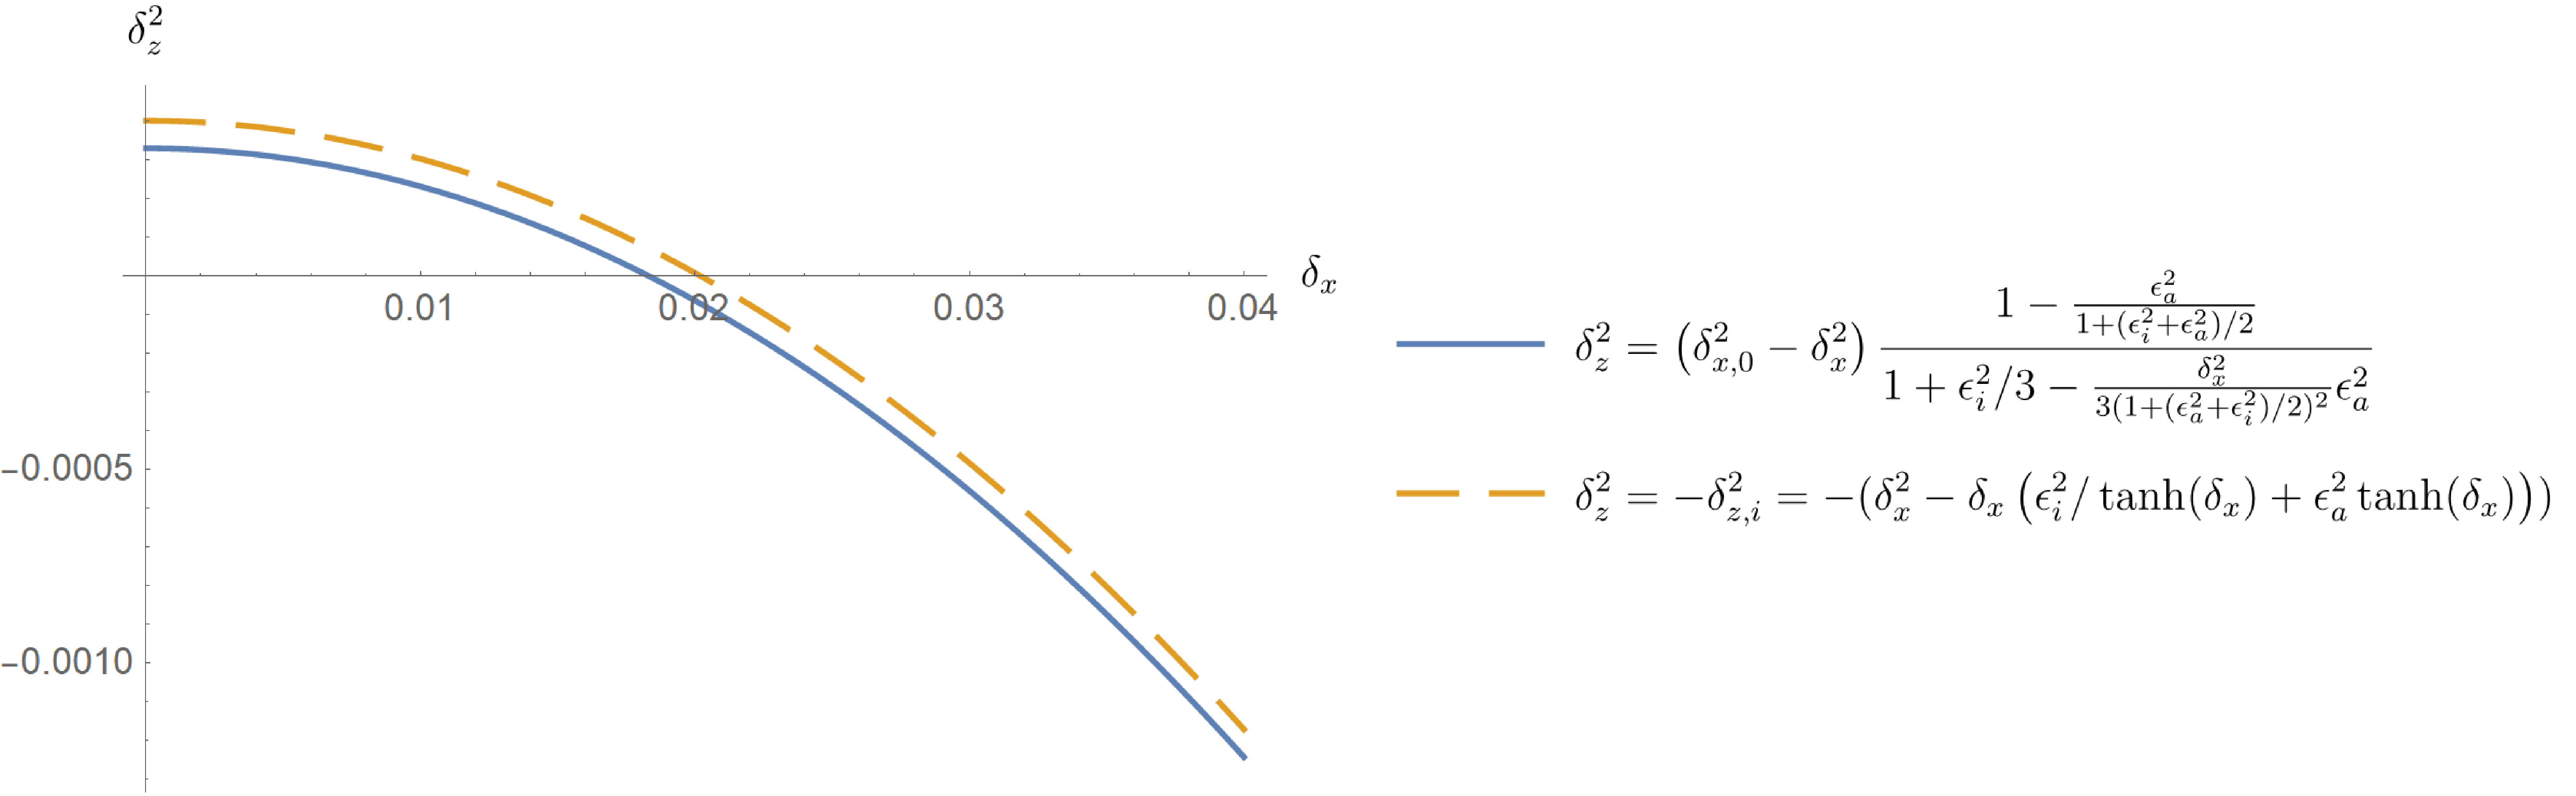
\includegraphics[width=0.9\linewidth]{FIGURES/dz2dx.png}
	}
\caption{Long waves: $\delta_z^2$ the square of the vertical wavenumber as a function of $\delta_x$ the horizontal wavenumber. The interval where $\delta_z^2$ is positive ($\delta_z$ real), for $\delta_x\le \delta_{x,0}$, corresponds to the barotropic mode while for $\delta_x\ge \delta_{x,0}$, $\delta_z^2$ is negative ($\delta_z$ purely imaginary) and this corresponds to the surface wave branch. The blue line is the accurate approximation given in \ref{deltazsurface} for long waves while the dashed orange curve corresponds to the approximation of surface waves given in \ref{longMSW}, this last approximation being more accurate for medium/short surface waves. The exact solution (not plotted), which can be numerically computed, is visually not distinguishable from the accurate blue curve.}
\label{dz2dx}
\end{figure}
\begin{figure}[h]
	\centerline{
		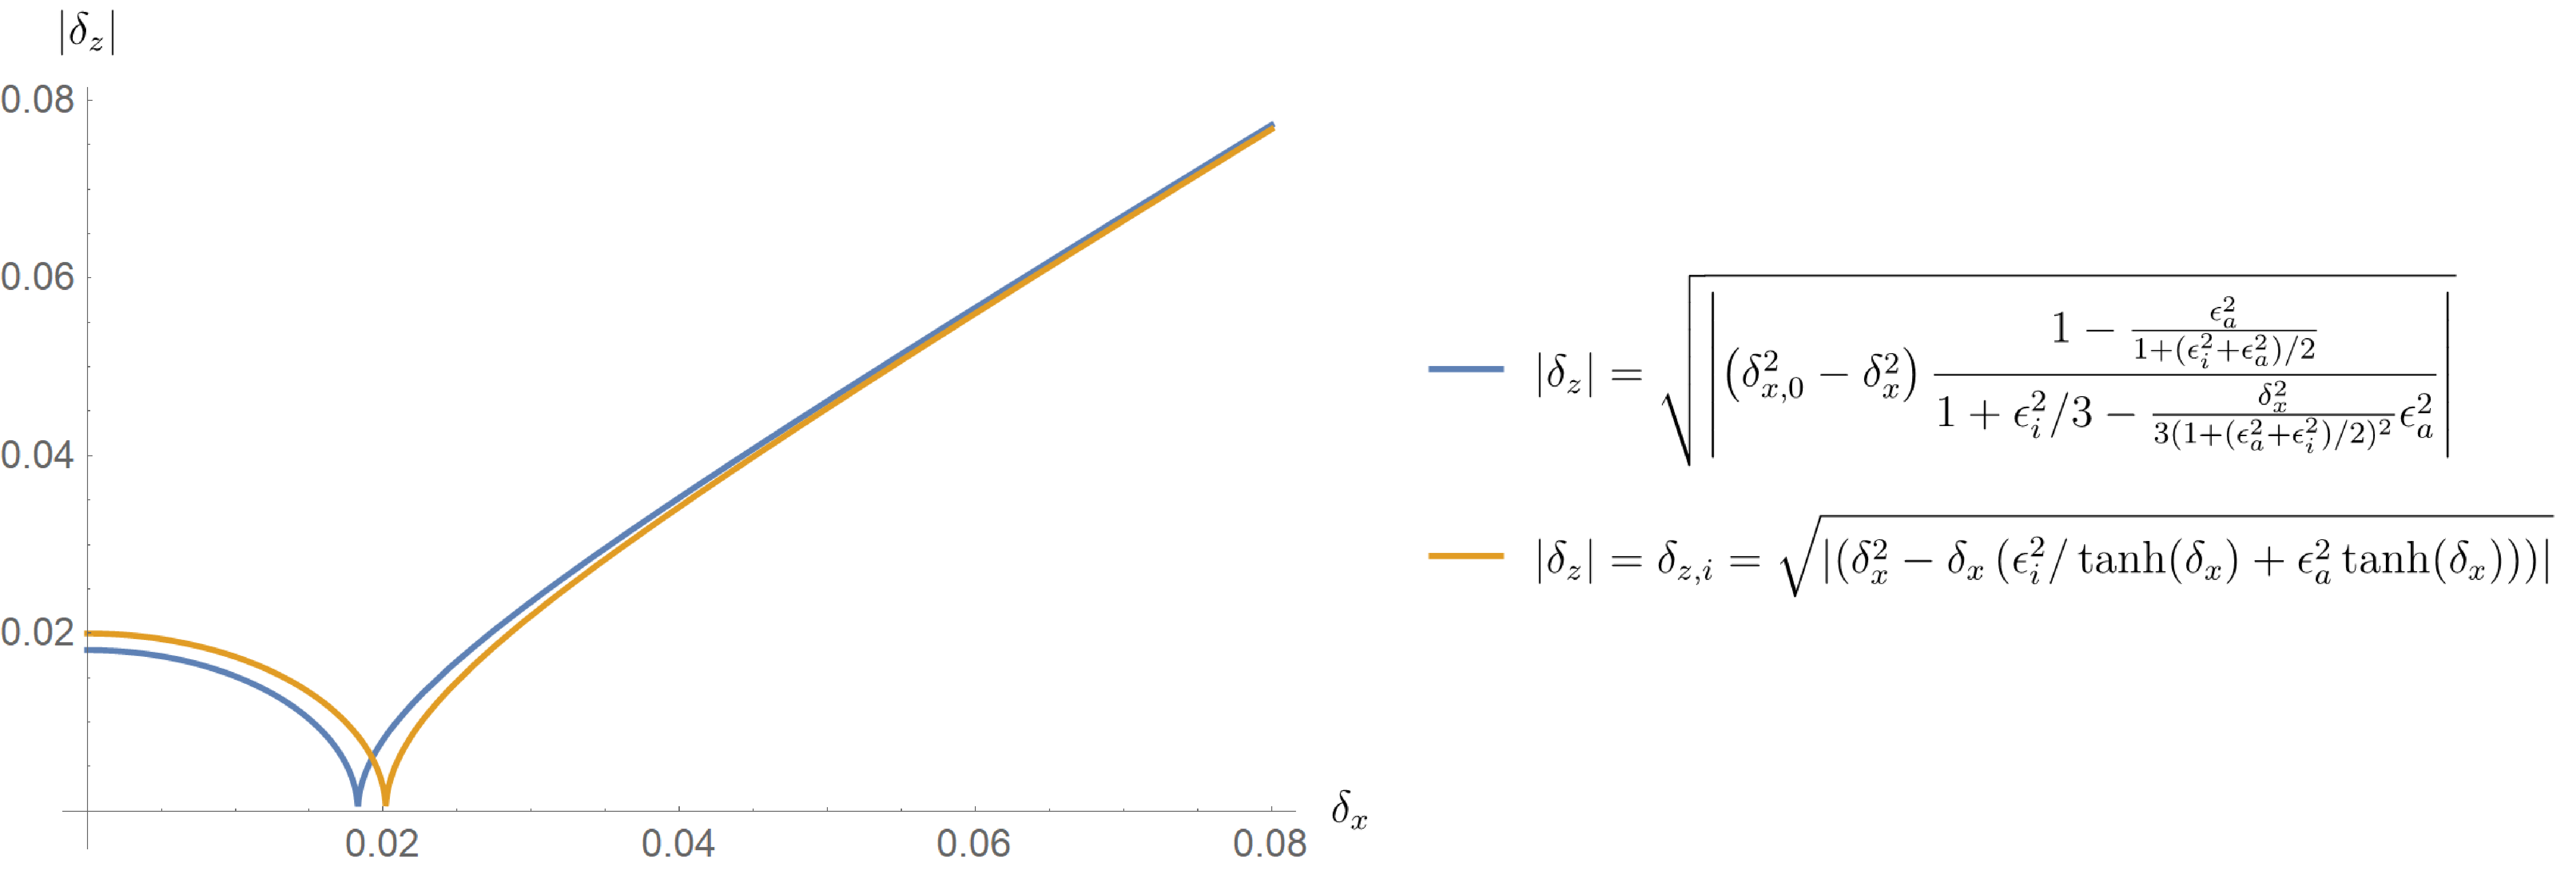
\includegraphics[width=0.9\linewidth]{FIGURES/dzdx.png}
	}
	\caption{Long waves: $|\delta_z|$ the modulus of the vertical wavenumber as a function of $\delta_x$ the horizontal wavenumber. The exact solution (not plotted), which can be numerically computed, is visually not distinguishable from the accurate blue curve. The vertical wavenumber of an incompressible and homogeneous ocean would correspond to the straight line $\delta_z=\delta_x$.}
	\label{dzdx}
\end{figure}
\\
%
%
Figure \oldref{omegadx} shows the values of the frequency $\omega$ as a function of the horizontal wavenumber $\delta_x$ according to different approximations. $\omega_{\mbox{\tiny Long Waves}}$ and $\omega_{\mbox{\tiny Medium Short Waves}}$ are computed by inserting the corresponding approximations \ref{deltazsurface} and \ref{longMSW} of $\delta_z$ in the boundary dispersion relation \ref{EqFullDisperb}. $\omega=\delta_x$ (resp. $\omega=\sqrt{\delta_x}$) is the classical long shallow water waves (resp. short non hydrostatic surface waves) approximation. $\omega=\sqrt{\delta_x \tanh(\delta_x)}$ is the frequency of an homogeneous and incompressible (non hydrostatic) ocean. Unsurprisingly, this last approximation is accurate over the full range of horizontal wavenumbers, even for the set of compressible stratified equations. Indeed, even if for long waves, $\delta_z$ is not directly linked to $\delta_x$ (in particular $\delta_z$ does not cancel for $\delta_x \approx 0$), $\delta_z$ remains small (less than $\epsilon_i$) and thus $\delta_z/\tan(\delta_z)$ is close to 1.
\begin{figure}[h]
	\centerline{
		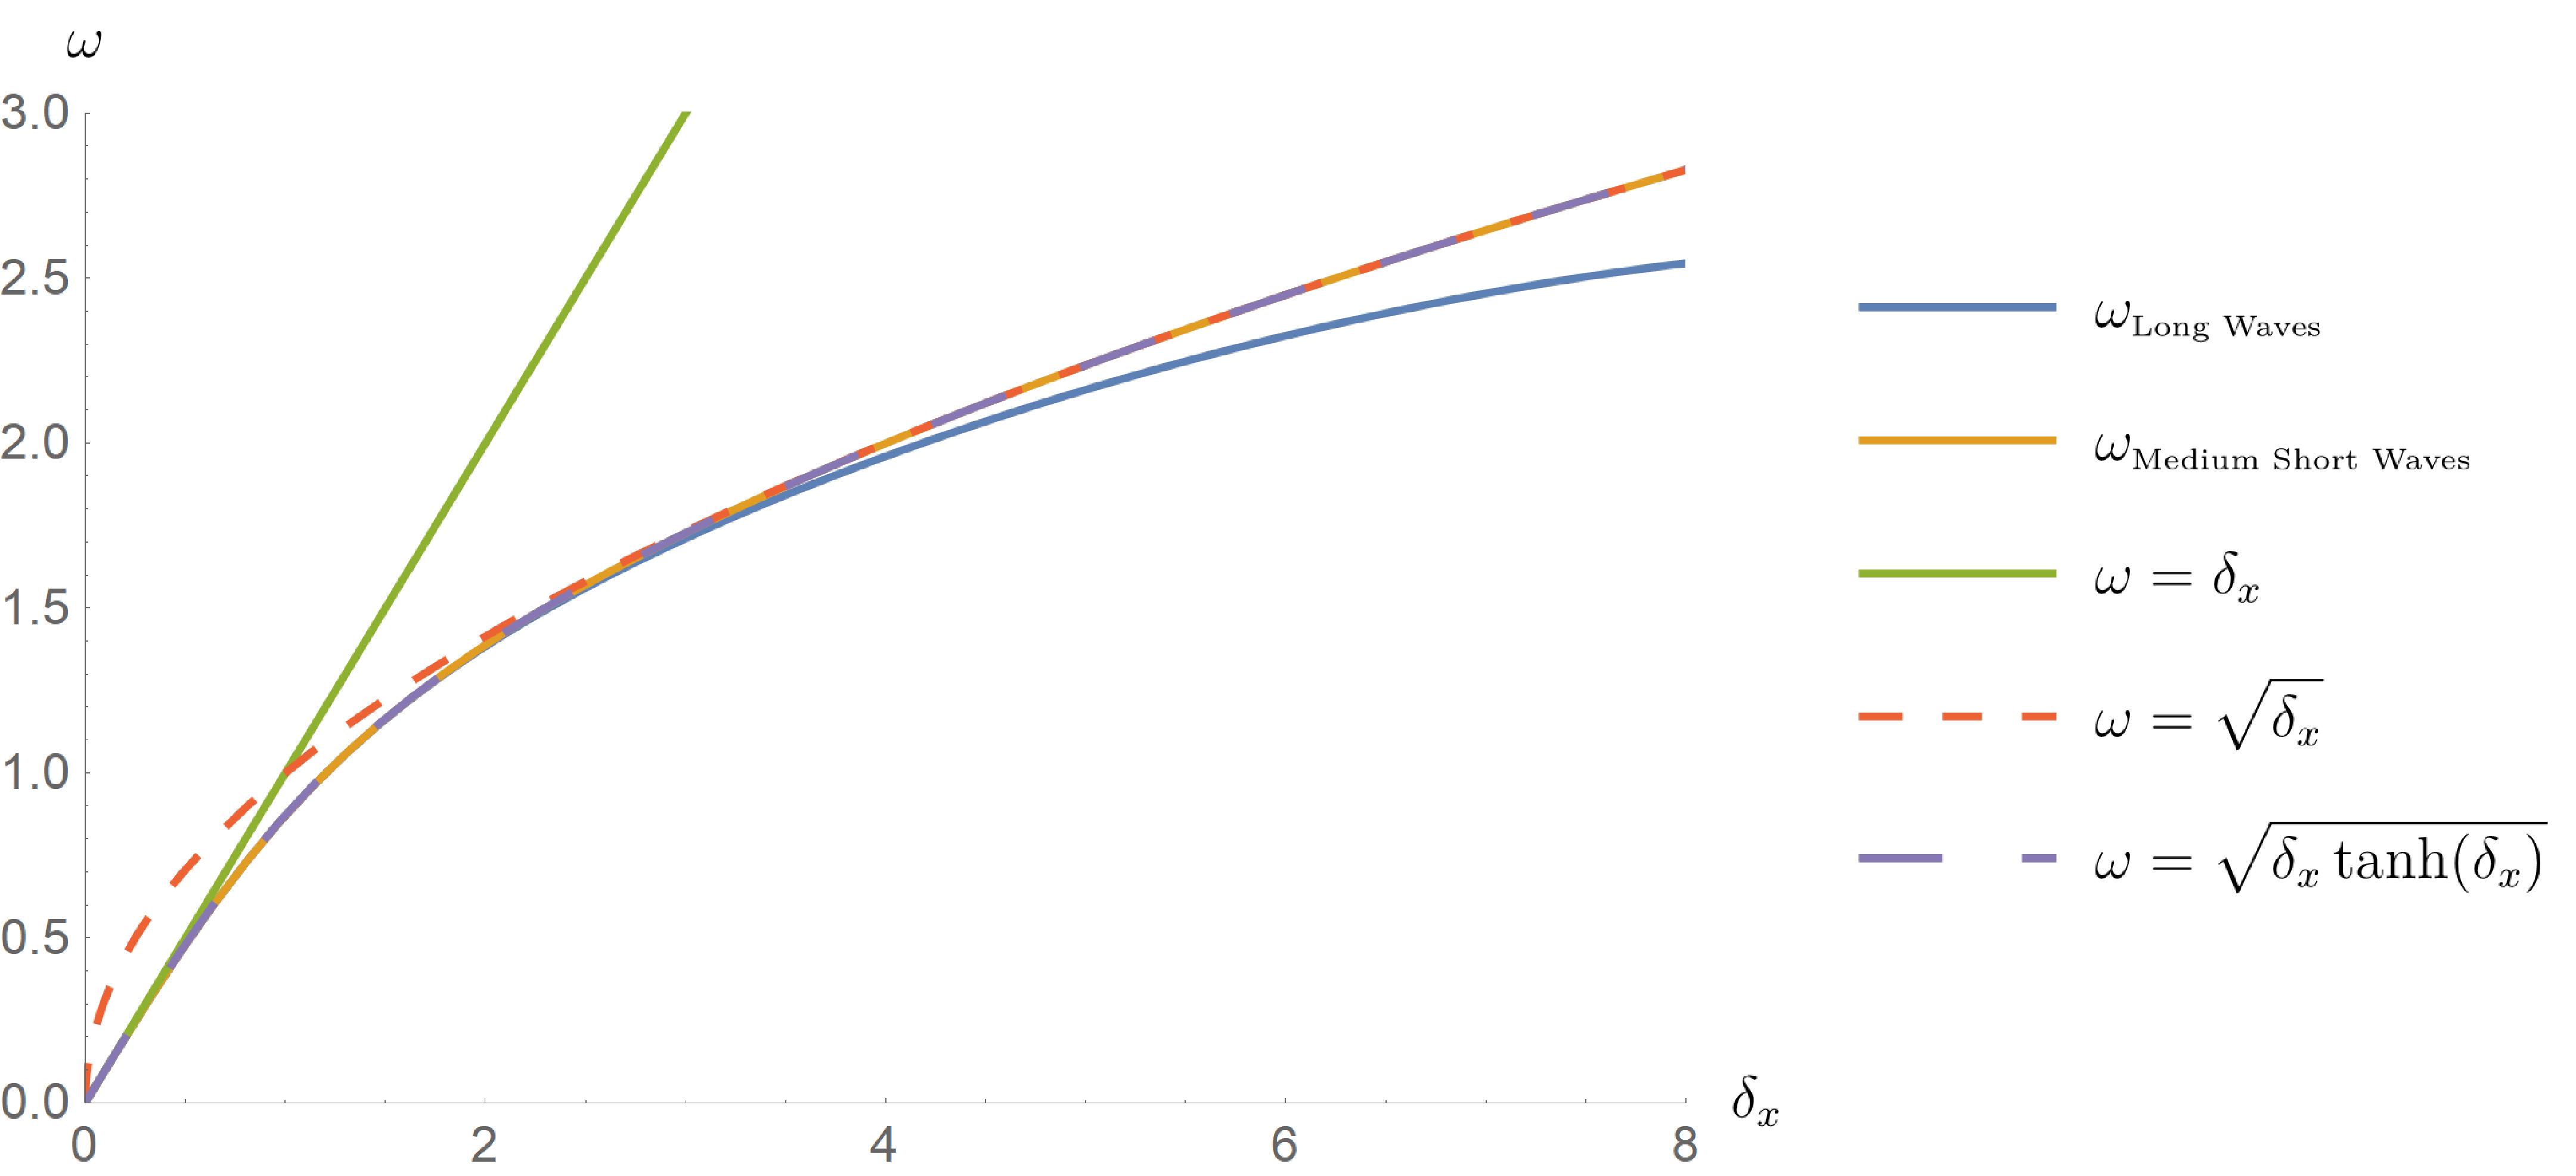
\includegraphics[width=0.9\linewidth]{FIGURES/omegadx.png}
	}
	\caption{Frequency $\omega$ as a function of $\delta_x$ the horizontal wavenumber for different approximations.}
	\label{omegadx}
\end{figure}


\textit{Orders of magnitudes:}\\
For the $4000m$-deep reference ocean (Table \oldref{TableParameters}), the horizontal length scale associated to the transformation of the MSW into the long MIM $(\lambda_{x,lmsw}=2\pi/(\delta_{x,lmsw}/4000))$ reaches $1367\ km$ against $62\ km$ for the same $10m$-deep ocean. When $\delta_x$ keeps on decreasing below $\delta_{x,lmsw}$, $\delta_z$ increases monotonically to a maximum value $\delta_{z,lmsw}(\delta_x=0)$. This vertical length scale reaches $1379\ km$ for the $4000m$-deep reference ocean and $62\ km$ for the same $10m$-deep ocean. The longer the horizontal length scale of the oscillation, the shorter the vertical length scale, and the weaker the stratification (vanishing $\epsilon_i$) the longer the horizontal length-scale $\lambda_{x,lmsw}$. This long MIM solution is a low-frequency oscillation of the ocean due to gravity and associated to the stratification of the ocean. It disappears when the stratification vanishes and the ocean can be assimilated to an homogeneous layer of water. It does persist in an incompressible ocean but is slightly modified by compressibility.

%\subsection{Close-to-singular MSW}
%
%The condition for propagation $(\displaystyle R^2(\delta_x,\delta_z)\le \frac{1}{4})$ derived in Section \ref{SubSectionFactoDisp} has so far been left out since for pulsations $\omega$ to remain real in the inner dispersion relation \ref{EqFullDispera}, it must necessarily be satisfied.  This condition is automatically satisfied for real horizontal and vertical wave-numbers but not necessarily for pure-imaginary vertical wave-numbers.\\
%A further question is to figure out if the resulting MSW wave solutions can or cannot approach and enter a region of the $(\delta_x,\ \delta_z,\ \omega)$ space where this condition is not satisfied. This would indeed lead to a pair of complex roots to \ref{solseq} and as a consequence to a wave solution diverging in time. Figure \ref{FigDelta} partially answers the question since it shows that the inner dispersion surface for pure-imaginary $\delta_z$ does not intersect the vertical (green) plane but remains tangent to it. We can show that the vertical component of the normal to the inner dispersion surface (i.e. $\partial$\ref{EqFullDisperai} $/\partial \omega$ ) vanishes for:
%\begin{equation}
%	   %\label{ParamAcousModes2}
%		\label{EqTurnPoints}
%		 \delta_x^2 - \delta_{z,i} ^2 
%		+\frac{(\epsilon_i^2+\epsilon_a^2)^2}{4}
%		-2 \epsilon_a^2 \omega^2 = 0
%\end{equation}
%	
%\begin{figure}[!h]
%	\centering		
%	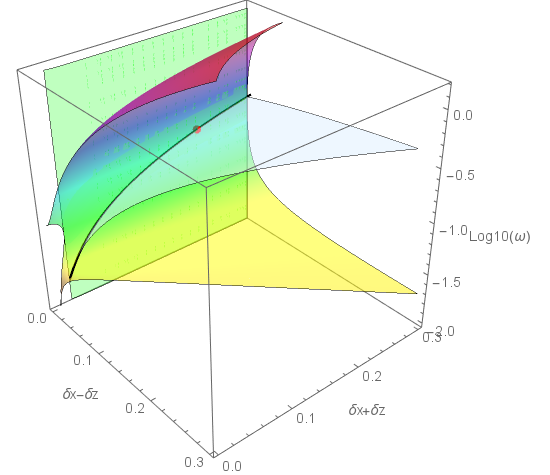
\includegraphics[width=0.5\linewidth]{FIGURES/Fig_Delta.png}
%	\caption{\textit{region of SMW close to instability (pure-imaginary vertical wave-number). Polychrome: inner dispersion surface. Light-blue: boundary dispersion surface. Light-green: vertical surface tangent to the inner dispersion surface. Red point: SMW solution close to instability. }}
%	\label{FigDelta}
%\end{figure}
%
%
%This set of points of the inner dispersion surface satisfies $\displaystyle R^2(\delta_x,i \delta_{z,i})= \frac{1}{4}$ and, as a consequence,
%$\omega^2=\omega_a^2/2$. They correspond to the black line on Figure \ref{FigDelta}. This line separates the inner dispersion surface in two parts: the upper acoustic region $(\omega^2\approx\omega_a^2)$ closer to the MAM branch and the lower region $(\omega^2\approx\omega_i^2)$ closer to the MIM region.\\
%If solutions to \ref{EqTurnPoints} and \ref{EqFullDisperai} can be found, at least one MSW wave intersects this line of points in phase-space. Such an intersection exists if there exist at least one point belonging to the boundary dispersion surface given by \ref{EqFullDisperb} or equivalently if the system of equations \ref{EqTurnPoints}, \ref{EqFullDisperai} and \ref{EqFullDisperb} has a solution. Only one single point satisfies this system, it is indicated by a large red dot on \ref{FigDelta}. Its horizontal and vertical wave-numbers can be expressed as functions of its pulsation:
%\begin{subequations}
%	\begin{alignat}{2}	
%	   \label{ParamSolDelta}
%	   &\delta_{z,i}(\omega) && =\frac{1}{2} 
%	   \sqrt{(\epsilon_i^2+\epsilon_a^2)^2 
%	   - 8 \epsilon_a^2 \omega^2
%	   + 4 \frac{\epsilon_a^2}{\epsilon_i^2} \omega^4}\\[3mm]
%	   &\delta_x(\omega) &&=\omega
%	   \sqrt{\frac{\epsilon_a^2+\epsilon_i^2}{2}
%	   +\delta_{z,i}(\omega)\ coth(\delta_{z,i}(\omega))}
%	\end{alignat}
%\end{subequations}
%The pulsation $\omega$ must then be a solution of the (transdental) equation inherited from the inner dispersion relation \ref{EqFullDisperai}:
%\begin{subequations}
%	\begin{alignat}{2}	
%	   \label{ParamSolDelta2}
% 		\delta_x^2(\omega)-\delta_{z,i}^2(\omega) 
% 		-\epsilon_i^2\ \frac{\delta_x^2(\omega)}
% 			{\omega^2}-\epsilon_a^2\omega^2
% 		+\frac{\epsilon_a^2+\epsilon_i^2}{4} = 0
%	\end{alignat}
%\end{subequations}
%For the parameters $\epsilon_i$ and $\epsilon_a$ given in Table \ref{TableParameters}, this latter equation has only one solution for $\omega^*$ satisfying the system of equations \ref{EqTurnPoints}, \ref{EqFullDisperai} and \ref{EqFullDisperb}. It can be evaluated numerically:
%\begin{equation}
%	\omega_* \approx 0.154
%\end{equation}
%Orders of magnitude of the wave-numbers $(\delta_{x,*},\ \delta_{z,*})$ and pulsations $(\omega_*)$ are given in Table \ref{TableOrdersMag}. The resulting wave solution is a MSW wave that satisfies $R^2(\delta_{x,*},\ \delta_{z,*})=1/4$. Graphically this means that the solution point (in red) belongs to the line of points with horizontal normal vector or vanishing vertical gradient with respect to $\omega$. Dynamically, this means that the corresponding wave solution is "on the edge" and that for a small variation of the wave-number, of the pulsation or one the parameters it may enters in the region of unstable waves satisfying $R^2>1/4$. \\
%Other reference parameters given in Table \ref{TableParameters} remaining constant, Table \ref{TableOrdersMag} shows that when changing the depth of the reference ocean (4000 m) to only 10 m, the (normalized) pulsation $\omega_*$ remains quasi-constant and, as a consequence, the pulsation $\Omega_*$ varies approximately with $0.154 \sqrt{g/H}$ in this range of parameters ($\Omega_*$ decreases thus from $12\ mn$ to only $41.3\ s$).


\subsection{Summary: waves solutions in a bounded ocean}
Table \oldref{TableWavesolutions_boundedmodified} summarizes the main results of this paper. The approximation for the different kind of waves (acoustic, gravity and surface waves/modes) are indicated in their dimensional form. For sake of readability, some of the relations given in Table \oldref{TableWavesolutions_boundedmodified} are lower order version of what has been proved previously. Most of the time, its corresponds to taking into account  the first-order correction terms only, in comparison to usual dispersion relation introduced in Table \oldref{TableWave solutions}. In that case, a red link to the higher approximation is given.
\begin{table}[!h]
	\centerline{
			\setlength{\extrarowheight}{30pt}
		\rotatebox{90}{
		\begin{tabular} {p{3.0cm}|p{8.6cm}|p{8cm}}
			Waves &  Frequency $(\Omega)$ & Vertical wavenumber $k_z$\\\hline
\begin{minipage}{3cm}
Modified Acoustic Modes (MAM)\\
$\small k_{z,m}=\frac{1}{H}(\pi/2+m\pi), m\ge 0$\\
\ref{SubSectionGraphicMAW}
\end{minipage}&
			$\displaystyle \Omega_{mam}^2=c_s^2(k_x^2+k_z^2)
			\left[
			1-\frac{g}{Hc_s^2}\frac{k_x^2-k_{z,m}^2}{(k_x^2+k_{z,m}^2)^2}+\frac{N^2}{gH}\frac{1}{k_x^2+k_{z,m}^2}
			\right]$&
			$\displaystyle
			k_{z,m}
			\left[
			1-\frac{g}{Hc_s^2}\frac{k_x^2-k_{z,m}^2}{2(k_x^2+k_{z,m}^2)k_{z,m}^2}
			+\frac{N^2}{2gH^2}\frac{1}{k_{z,m}^3}
			\right]
			$\quad {\color{red}\ref{ParamallMAM1}}	
			\\[8mm] \hline
\begin{minipage}{3cm}
Modified Internal Modes (MIM)\\
$k_{z,n}=\frac{1}{H}(n\pi), m\ge 1$\\
\ref{SubSectionGraphicMIW}
\end{minipage}
& $\displaystyle \Omega_{mim}^2=\frac{N^2 k_x^2}{k_x^2+k_{z,n}^2}
			\left[
			1-2\frac{N^2}{gH}\frac{k_{z,n}^2}{(k_x^2+k_{z,n}^2)^2}
			\right]
			$
			&
			$\displaystyle
			k_{z,n}
			\left[
			1+\frac{N^2}{gH}
			\frac{1}{k_x^2+k_{z,n}^2}
			+\left(\frac{N^2}{gH}\right)^3
\frac{(k_x^2-k_{z,n}^2)}{(k_x^2+k_{z,n}^2)^3}
			\right]
			$		\\[8mm] \hline
\begin{minipage}{3cm}
Barotropic mode\\
$k_x\le k_{x,0}\approx \frac{N^2}{g}$\\
\ref{SubSectionLongWavesrealdz}
\end{minipage}&
$\Omega^2 = gHk_x^2 \left[
1
-\frac{1}{6}\left(
\epsilon_i^2+3\epsilon_a^2
\right)
\right]$\qquad {\color{red}\ref{eqomegalongwavereal}}&
$\displaystyle \sqrt{k_{x,0}^2-k_x^2}$
\qquad
{\color{red}\ref{deltazsurface}}
\\[8mm] \hline
\begin{minipage}{3cm}
Long\\
surface waves\\
$k_x\ge k_{x,0}\approx \frac{N^2}{g}$\\
\ref{SubSectionLongWavesrealdz}
\end{minipage}
&$\Omega^2 = gHk_x^2 \left[
1
-\frac{1}{6}\left(
\epsilon_i^2+3\epsilon_a^2
\right)
\right]$\qquad {\color{red}\ref{eqomegalongwavereal}}&
$\displaystyle i\sqrt{k_x^2-k_{x,0}^2}$
\qquad
{\color{red}\ref{deltazsurface}}
\\[8mm] \hline
\begin{minipage}{3cm}
Medium and short\\
surface waves\\
$k_x\ge k_{x,0}\approx \frac{N^2}{g}$
\\
\ref{SubSectionGraphicMSW}
\end{minipage}
&
$\displaystyle
\Omega^2=
gk_x\tanh(Hk_x)$
\qquad
{\color{red}\ref{eqomegasurfacewaves}}
&
$\displaystyle i k_x \sqrt{1-\frac{1}{k_x}\left(
\frac{N^2}{g\tanh(Hk_x)}
+
\frac{g}{c_s^2}\tanh(Hk_x)
\right)}$
	\end{tabular}}}
	\caption{{\color{red}corriger legende ...}Compressibility and stratification induced modifications to the usual dispersion relations given in table \ref{TableWave solutions}. $\Omega$ is wave angular frequency, $k_x$ and $k_z$ are the wavenumbers, $g$ is the acceleration of gravity, $N$ a reference Brunt-V\"ais\"al\"a frequency and $c_s$ the speed of sound. $D_0$ is the background density vertical scale and is given by $1/D_0=N^2/g+g/c_s^2$}
	\label{TableWavesolutions_boundedmodified}
\end{table}
\newpage
{\color{red}FIN MODIFS LAURENT}
%%%%%%%%%%%%%%%%%%%%%%%%%%%
% Table order of magnitude
%%%%%%%%%%%%%%%%%%%%%%%%%%%
\begin{table}[h]
	%\centerline{
	\begin{tabular}{l|l|l|l|l}
		& \textit{Notation}   & \textit{Reference} & \textit{10-m-deep} & \textit{$N=10^{-2}\ s^{-1}$}\\\hline
		Parameters & $\epsilon_a$ &
		$0.13$ &
		$6.6\  10^{-3}$ & $0.13$\\
		& $\epsilon_i$ &
		$2.0\ 10^{-2}$ &
		$1.0\ 10^{-3}$ & $0.20$\\\hline
		\specialrule{0pt}{2pt}{0pt}
		Acoustic cut-off&$2\pi \sqrt{H/g} /\omega_{c,a}$ & $30\ mn$ & $30\ mn$ & $9.6\ mn$\\\hline
		\specialrule{0pt}{2pt}{0pt}
		Internal cut-off& $2\pi \sqrt{H/g} /\omega_{c,i}$& $1.7\ h$ & $1.7\ h$ & $10.5\ mn$\\\hline
		\specialrule{0pt}{2pt}{0pt}
		LMIM-LMSW cut-off & $2\pi H/\delta_{x,0}$& $1367\ km$ & $1000\ km$ & $123\ km$\\
		& $2\pi \sqrt{H/g} \omega_{x,0}$ & $1.9\ h$ & $1.7\ h$ & $10.5\ mn$\\\hline
		\specialrule{0pt}{2pt}{0pt}
		LMIM-$\delta_z(0)$ & $2\pi H/\delta_{z,0}$& $1379\ km$ & $62\ km$& $125\ km$\\
		& $2\pi \sqrt{H/g} \omega_{z,0}$ & $\infty$& $\infty$ & $\infty$\\ \hline
		\specialrule{0pt}{2pt}{0pt}
		MSW-neutral point & $2\pi H/\delta_{x,*}$& $161\ km$ & $407\ m$ & $123\ km$\\
		&$2\pi H/\delta_{z,*}$ & $164\ km$ & $407\ m$&$2148\ km$\\
		&$2\pi \sqrt{H/g} \omega_{*}$ &$12\ mn$&$41.3\ s$&$10.5\ mn$\\
	\end{tabular}
	%}
	\caption{orders of magnitude of various scales. Notations refer to non-dimensional variables whereas orders of magnitude are given for dimensional quantities. Parameters for the "\textit{Reference}" ocean are given in Table \ref{TableParameters}. "\textit{10-m-deep}" ocean is a  10-m-deep \textit{Reference} ocean and "$N=10^{-2}\ s^{-1}$" refers to a \textit{"Reference"} ocean with $N=10^{-2}\ s^{-1}$.} 
	\label{TableOrdersMag}
\end{table}